\documentclass[11pt]{amsart}
\usepackage[all]{xy}
\usepackage[dvips]{graphicx}
\usepackage{amsfonts}
\usepackage{amssymb,latexsym,amsmath}
\usepackage{amsthm}
\usepackage{color}
\usepackage{empheq}
\usepackage{float}
\usepackage{hyperref}
\usepackage{listings}
\usepackage{mathrsfs}
\usepackage{slashed}
\usepackage{tikz}

\definecolor{dkgreen}{rgb}{0,0.6,0}
\definecolor{gray}{rgb}{0.5,0.5,0.5}
\definecolor{mauve}{rgb}{0.58,0,0.82}

\newtheorem{remark}{Remark}

\lstset{frame=tb,
    language=python,
    aboveskip=3mm,
    belowskip=3mm,
    showstringspaces=false,
    columns=flexible,
    basicstyle={\small\ttfamily},
    numbers=left,
    numberstyle=\tiny\color{gray},
    keywordstyle=\color{blue},
    commentstyle=\color{dkgreen},
    stringstyle=\color{mauve},
    breaklines=true,
    breakatwhitespace=true,
    tabsize=3
}

\textwidth = 420pt
\oddsidemargin = 18pt
\evensidemargin = 18pt

\begin{document}
\title{Cohort Revenue \& Retention Analysis: A Bayesian Approach}
\author{Juan Camilo Orduz}
\email{juanitorduz@gmail.com}
\urladdr{\href{https://juanitorduz.github.io/}{https://juanitorduz.github.io/}}
\address{Berlin, Germany}
\date{\today}

\begin{abstract}
We present a bayesian approach to model cohort-level retention rates and revenue over
time. We use bayesian additive regression trees (BART) to model the retention
component which we couple with a linear model to model the revenue component.
This method is flexible enough to allow adding additional covariates to both model
components. This bayesian model allows us to quantify the uncertainty in the
estimation, understand the effect of the covariates on the retention through partial
dependence plots (PDP), individual conditional expectation (ICE) plots and last but not
least forecast the future revenue and retention rates.
\end{abstract}

\maketitle

\tableofcontents

\section{Introduction}

Retention and customer lifetime value estimation are one of the most important aspects
to understand customer behavior. There are many ways to model retention and revenue 
by modeling individual-level purchase behavior for both the contractual and the
non-contractual setting, see for example the work by Fader and Herdie
\cite{FaderHardie2007} and \cite{FaderHardie2005} respectively\footnote{Our definition
of retention is what they call survival curve. See precise definitions below.}. In real
cases, one is interested in modeling retention and revenue at cohort-level. There are
(at least) three options to use the techniques mentioned above to model cohort-level
retention:

\begin{enumerate}
    \item Pool the cohorts together and model the retention and revenue as a whole.
    \item Un-pool the cohorts and model each cohort separately.
    \item Try to model the cohorts jointly.
\end{enumerate}

See \cite{FaderHardieNote2017} for more details on these approaches. One of the
limitations of those approaches is that they are not flexible enough to model
seasonality and add external regressors\footnote{Actually, one can add regressors in
some cases as described in \cite{FaderHardieNote2007} in the non-contractual case.}.
One can argue that seasonality is not that important when trying to estimate the
customer-lifetime-value. Nevertheless, in practice, there are business models on which
the customer base is very seasonal. \\

In this work, we present a bayesian approach to model cohort-level retention rates from
a top-down perspective. We do not model the individual-level purchase
behavior\footnote{This is a clear limitation if one is interested at customer-level
parameters and predictions.} but rather the retention and revenue at cohort matrices.
This approach allows for modeling non-linear relationships between cohorts, adding
seasonality and external regressors. Concretely, we use bayesian additive regression
trees (BART, see \cite{quiroga2022bart}) to model the retention component and we couple
it with a linear model to model the revenue. The following are the main ingredients 
behind the model:


\subsection*{Features}
The following are the main features used to model retention and revenue:
\begin{itemize}
    \item {\bf Cohort age}: Age of the cohort in months.
    \item {\bf Age}: Age of the cohort with respect to the observation time.
        This feature is a numerical encoder for the cohort.
    \item {\bf Month}: Month of the observation time.
\end{itemize}

In Figure \ref{fig:retention_matrix} we show an example of a retention matrix. Note
that we are removing the diagonal as it is not informative since it has just ones. As
an example, let us assume our observation month is {\em 2022-11} and consider the cohort
{\em 2022-09}. In this case, the age of this cohort is $2$ months as it is always
relative to the observation period. This cohort was two observation periods
{\em 2022-10} and {\em 2022-11} with cohort age $1$ and $2$ respectively.\\

Note that all of these features are accessible for out-of-sample predictions.
As we will see below, in practice we can add more covariates to the model.
The only requirement for out-of-sample predictions is that the covariates are available
for the new observation period. \\

\begin{figure}
    \centering
    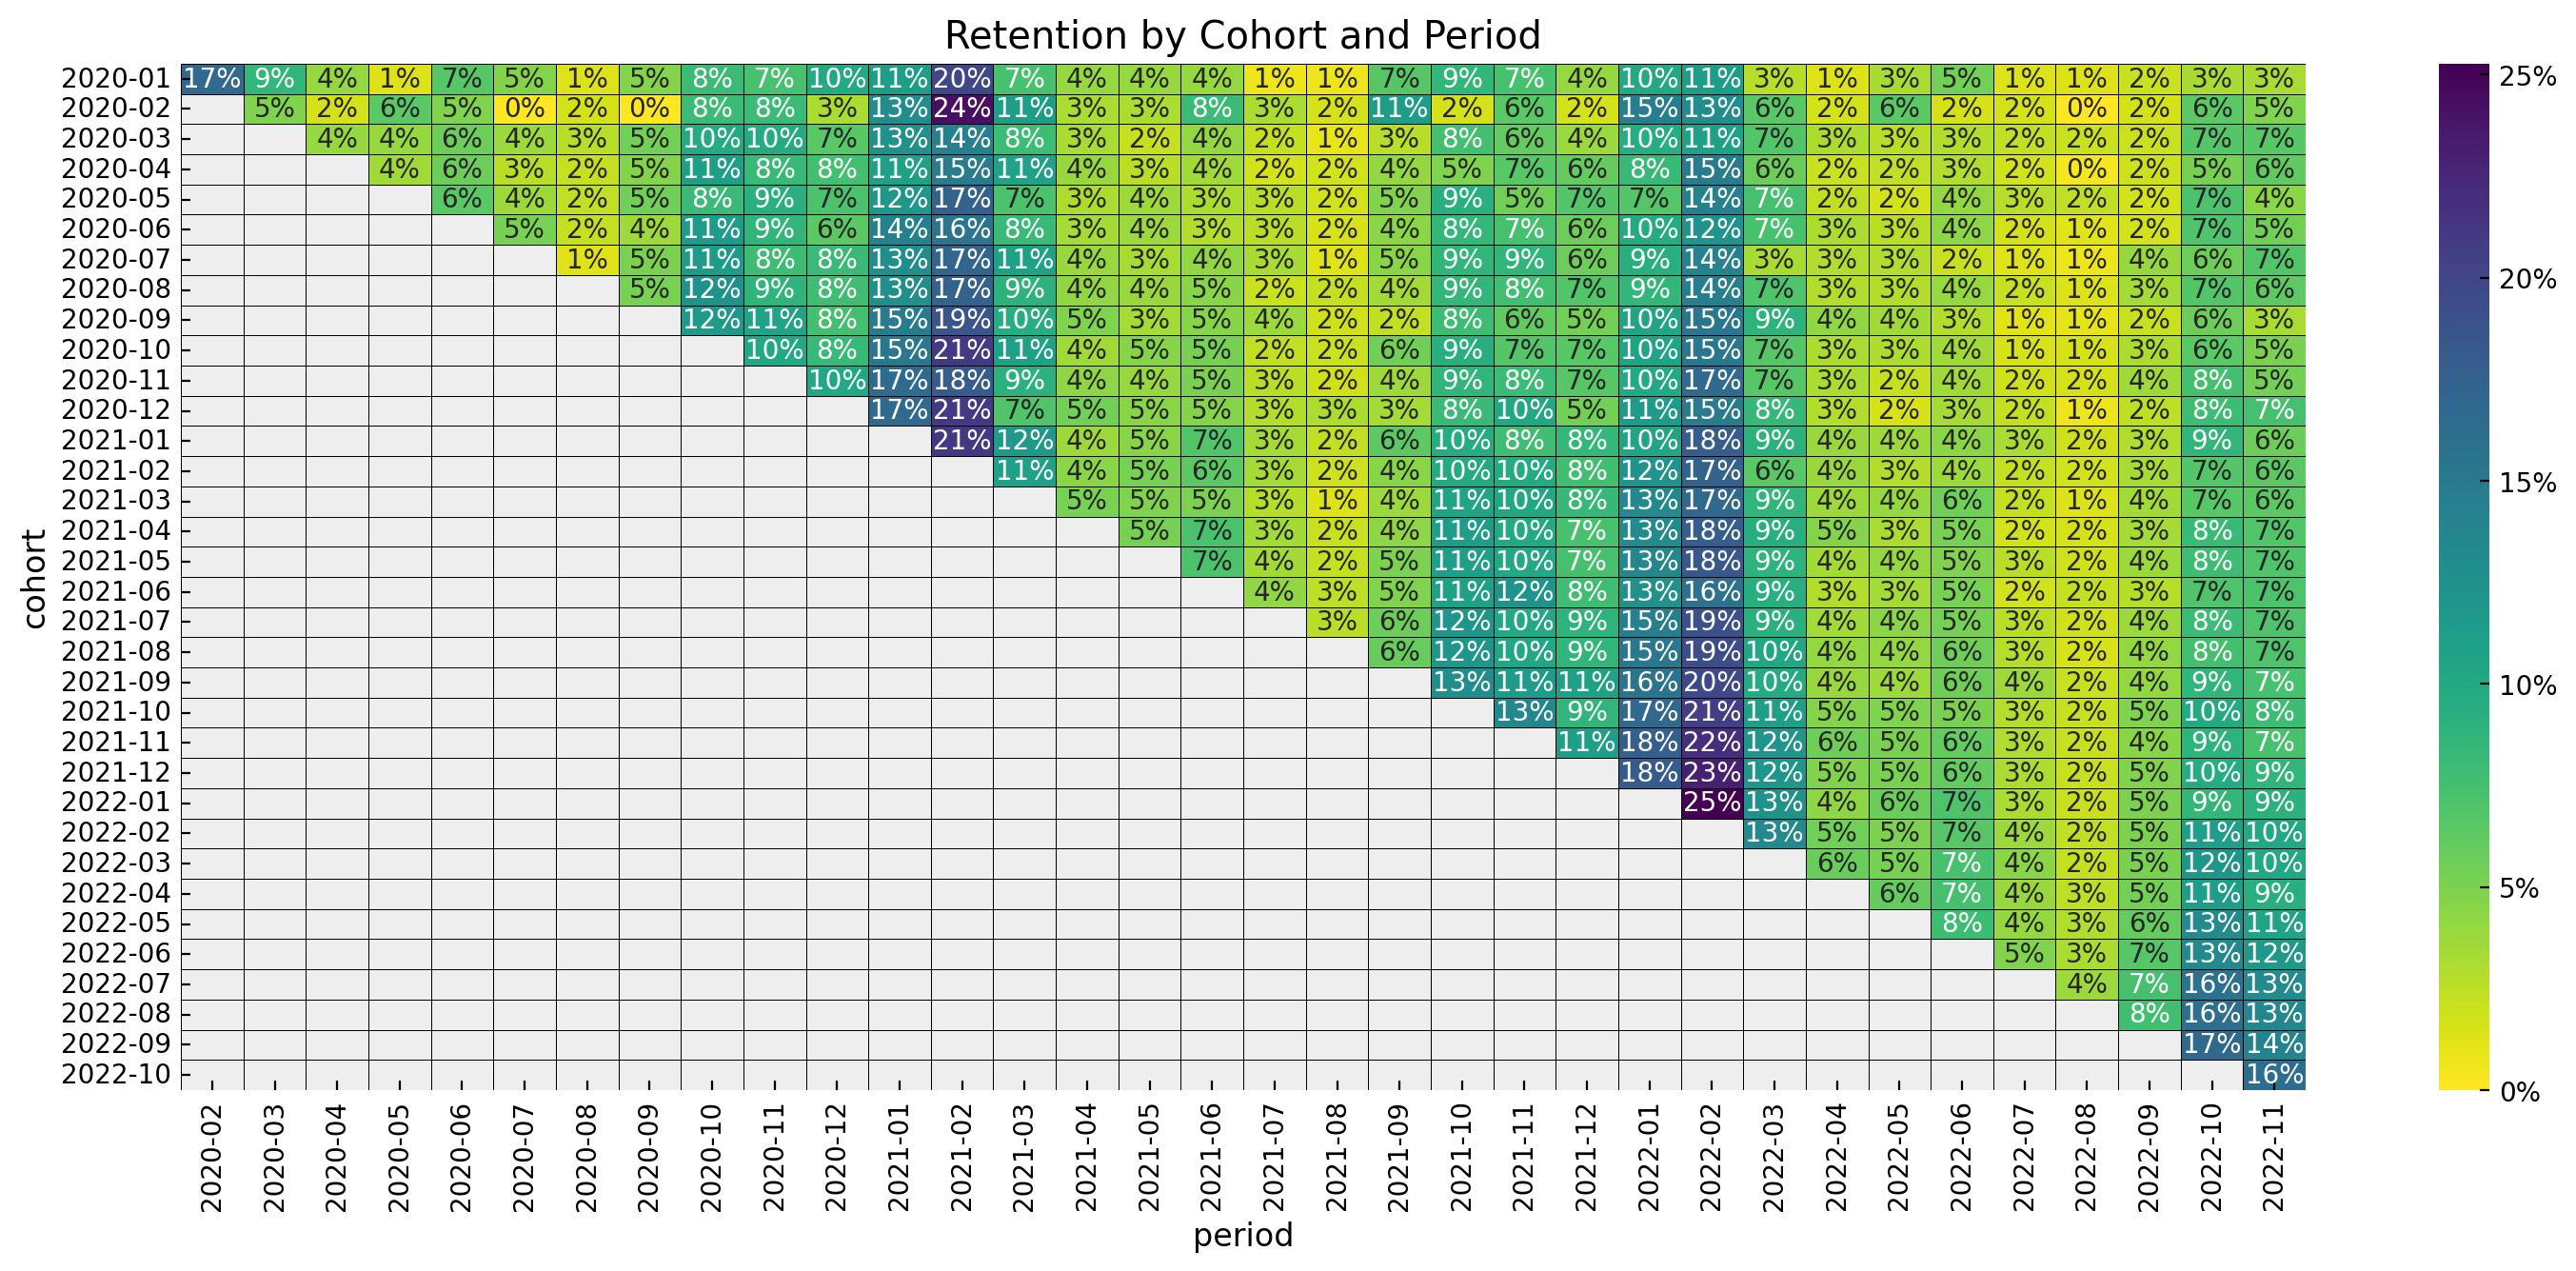
\includegraphics[width=\textwidth]{images/revenue_retention_17_0.png}
    \caption{Retention matrix example.}
    \label{fig:retention_matrix}
\end{figure}

\subsection*{Model Specification} 
\begin{itemize}
    \item We model the number of active users in the cohort as a binomial random
        variable $\text{Binomial}(N_{\text{total}}, p)$, where the parameter $p$
        represents the retention. We model the latent variable $p$ using a BART model
        with features cohort age, age and month.
    
    \item We model the revenue as a gamma random variable
        $\text{Gamma}(N_{\text{active}}, \lambda)$. We model the latent variable
        $\lambda$ through a linear model with features cohort age, age and a
        multiplicative interaction. Note that we do not add a seasonality component as
        we often see most of the seasonality coming from the retention itself. This of
        course can be added as a feature (plus any other covariates!) to the model.
    
    \item Here is a summary of how the retention and revenue components are coupled
        together:
    
    \begin{align*}
        \text{Revenue} & \sim \text{Gamma}(N_{\text{active}}, \lambda) \\
        \log(\lambda) = (& \text{intercept} \\
            & + \beta_{\text{cohort age}} \text{cohort age} \\
            & + \beta_{\text{age}} \text{age} \\
            & + \beta_{\text{cohort age} \times \text{age}} \text{cohort age} \times \text{age}) \\
        N_{\text{active}} & \sim \text{Binomial}(N_{\text{total}}, p) \\
        \textrm{logit}(p) & = \text{BART}(\text{cohort age}, \text{age}, \text{month})
    \end{align*}
    
\end{itemize}

We are interested in estimating the BART parameters and the beta coefficients (plus the
intercept) of the linear component simultaneously. Figure
\ref{fig:revenue_retention_model} summarizes the model structure.

\begin{figure}
    \centering
    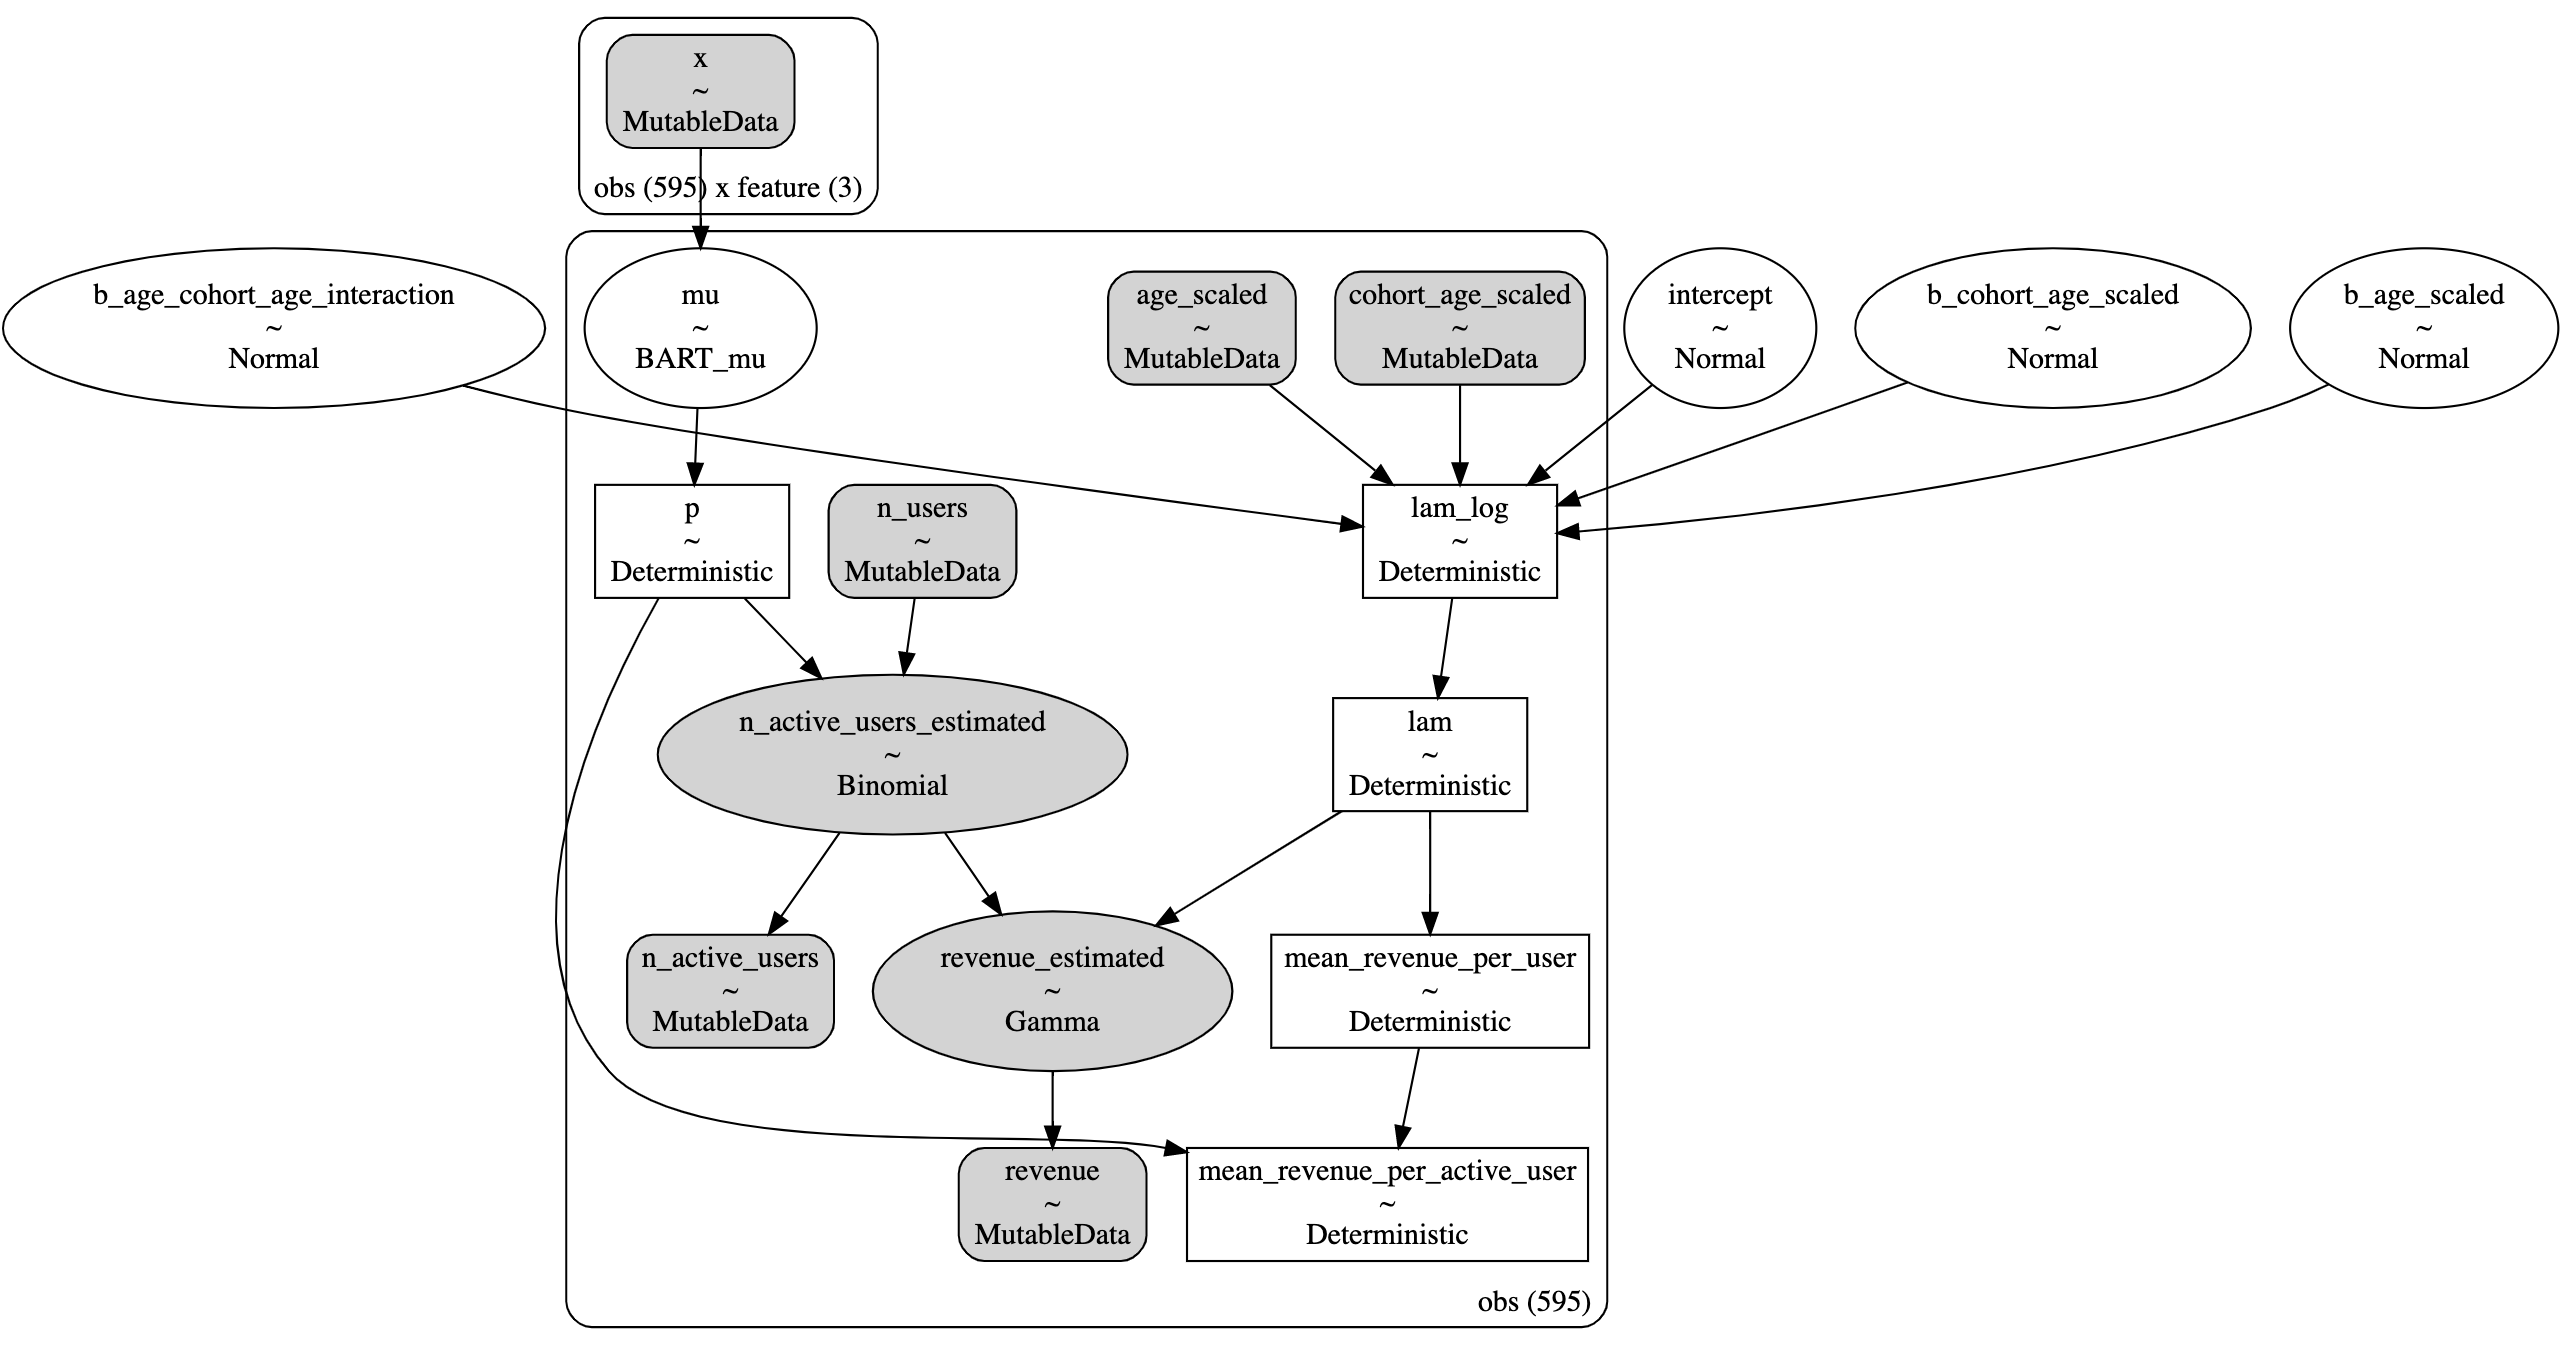
\includegraphics[width=\textwidth]{images/revenue_retention_33_0.png}
    \caption{Cohort-revenue-retention model structure.}
    \label{fig:revenue_retention_model}
\end{figure}


\begin{remark}
This work is the result of a sequence of blog posts where all the details on the code
and implementation are presented, see \cite{orduz_retention},
\cite{orduz_retention_bart} and \cite{orduz_revenue_retention}.  
\end{remark}


\section{Synthetic Data}

We illustrate the definitions, concepts and model using a synthetic data set (you can
get it as {\em csv} from \cite{orduz_revenue_retention_data}). The code to
(deterministically!) generate the data set is publicly available in 
\cite{orduz_revenue_retention_data_code}. \\

To start the analysis, let's do some exploratory data analysis. Figure
\ref{fig:retention_matrix} shows the retention matrix per cohort and period. There are 
two things to note at first glance:

\begin{enumerate}
    \item The retention has a clear seasonal pattern concerning the period. Note it is 
        higher in the last months of the year and lower in the middle of the year. To 
        see the seasonality pattern in a clearer way see Figure 
        \ref{fig:retention_seasonal}.
    \item The retention seems to be increasing as the age decreases. You could see this
    by comparing the retention values when the period month is November and the cohort
    age is one.
\end{enumerate}

\begin{figure}
    \centering
    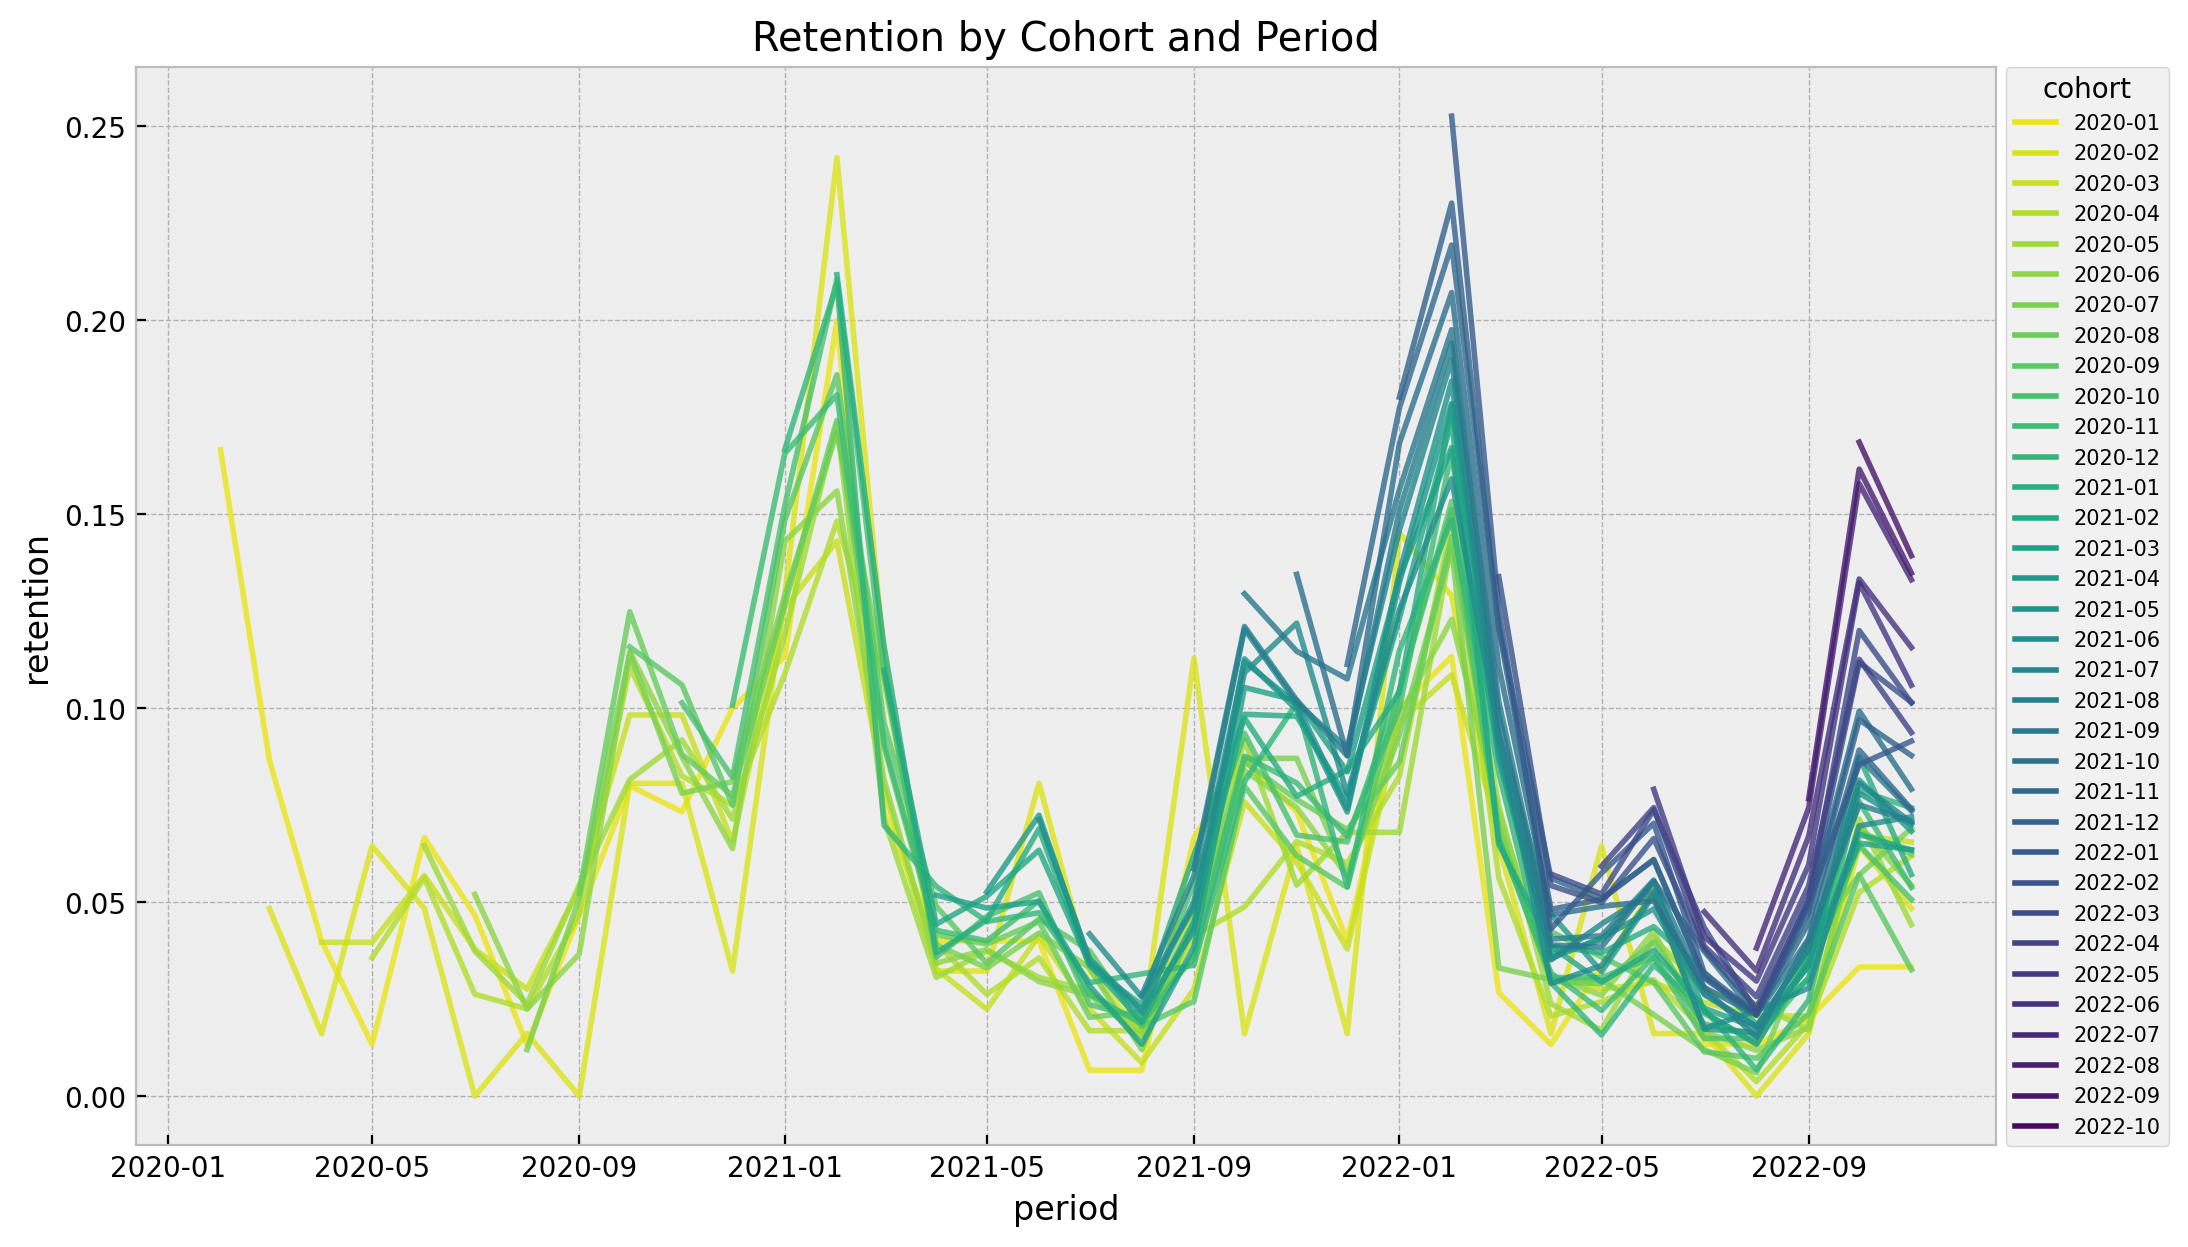
\includegraphics[width=\textwidth]{images/revenue_retention_19_0.png}
    \caption{Retention as a function of the period. This plot clearly shows the yearly
    seasonality pattern of the retention values.}
    \label{fig:retention_seasonal}
\end{figure}

It is important to keep in mind that the retention metric is a quotient, and therefore
the cohort size matters. For example, a retention rate of 0.4 could come from $4/10$ or
$4\times 10^{5} / 10^{6}$. One could argue that the former case carries more
uncertainty regarding the estimation. This motivates looking into the number of active
users' values. These are shown in Figure \ref{fig:active_users}. We can see that the
number of active users increases considerably for newer cohorts. We would like this
information to be encoded in the model. \\

\begin{figure}
    \centering
    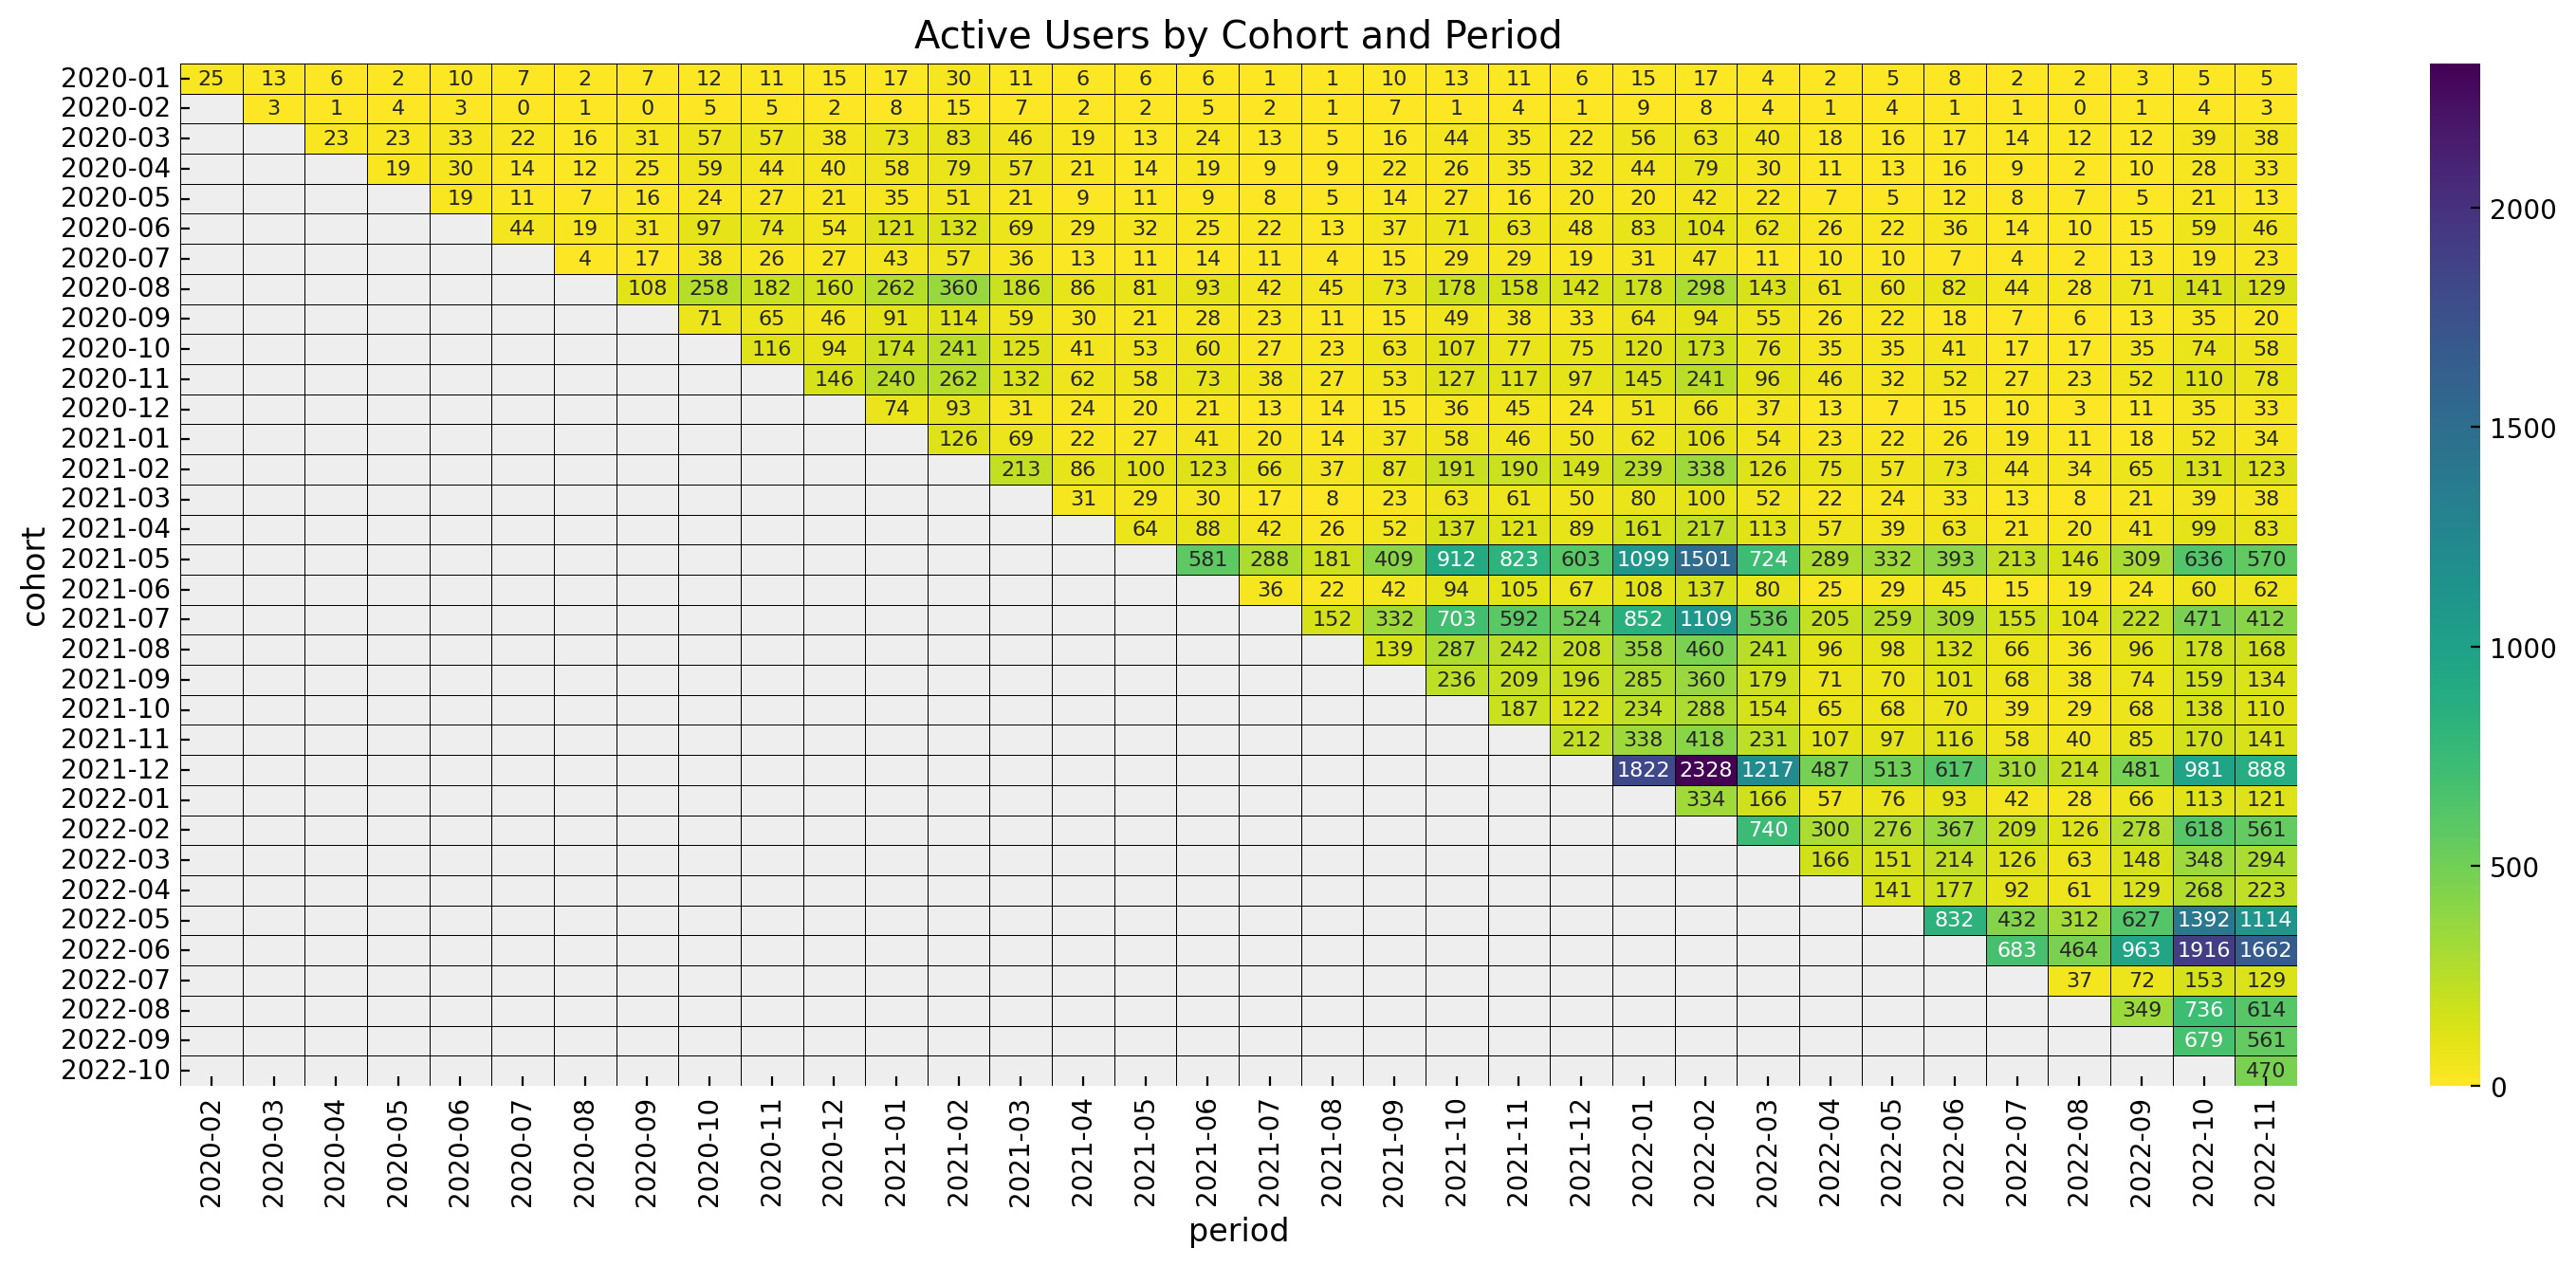
\includegraphics[width=\textwidth]{images/revenue_retention_21_0.png}
    \caption{Active users' values.}
    \label{fig:active_users}
\end{figure}

\begin{figure}
    \centering
    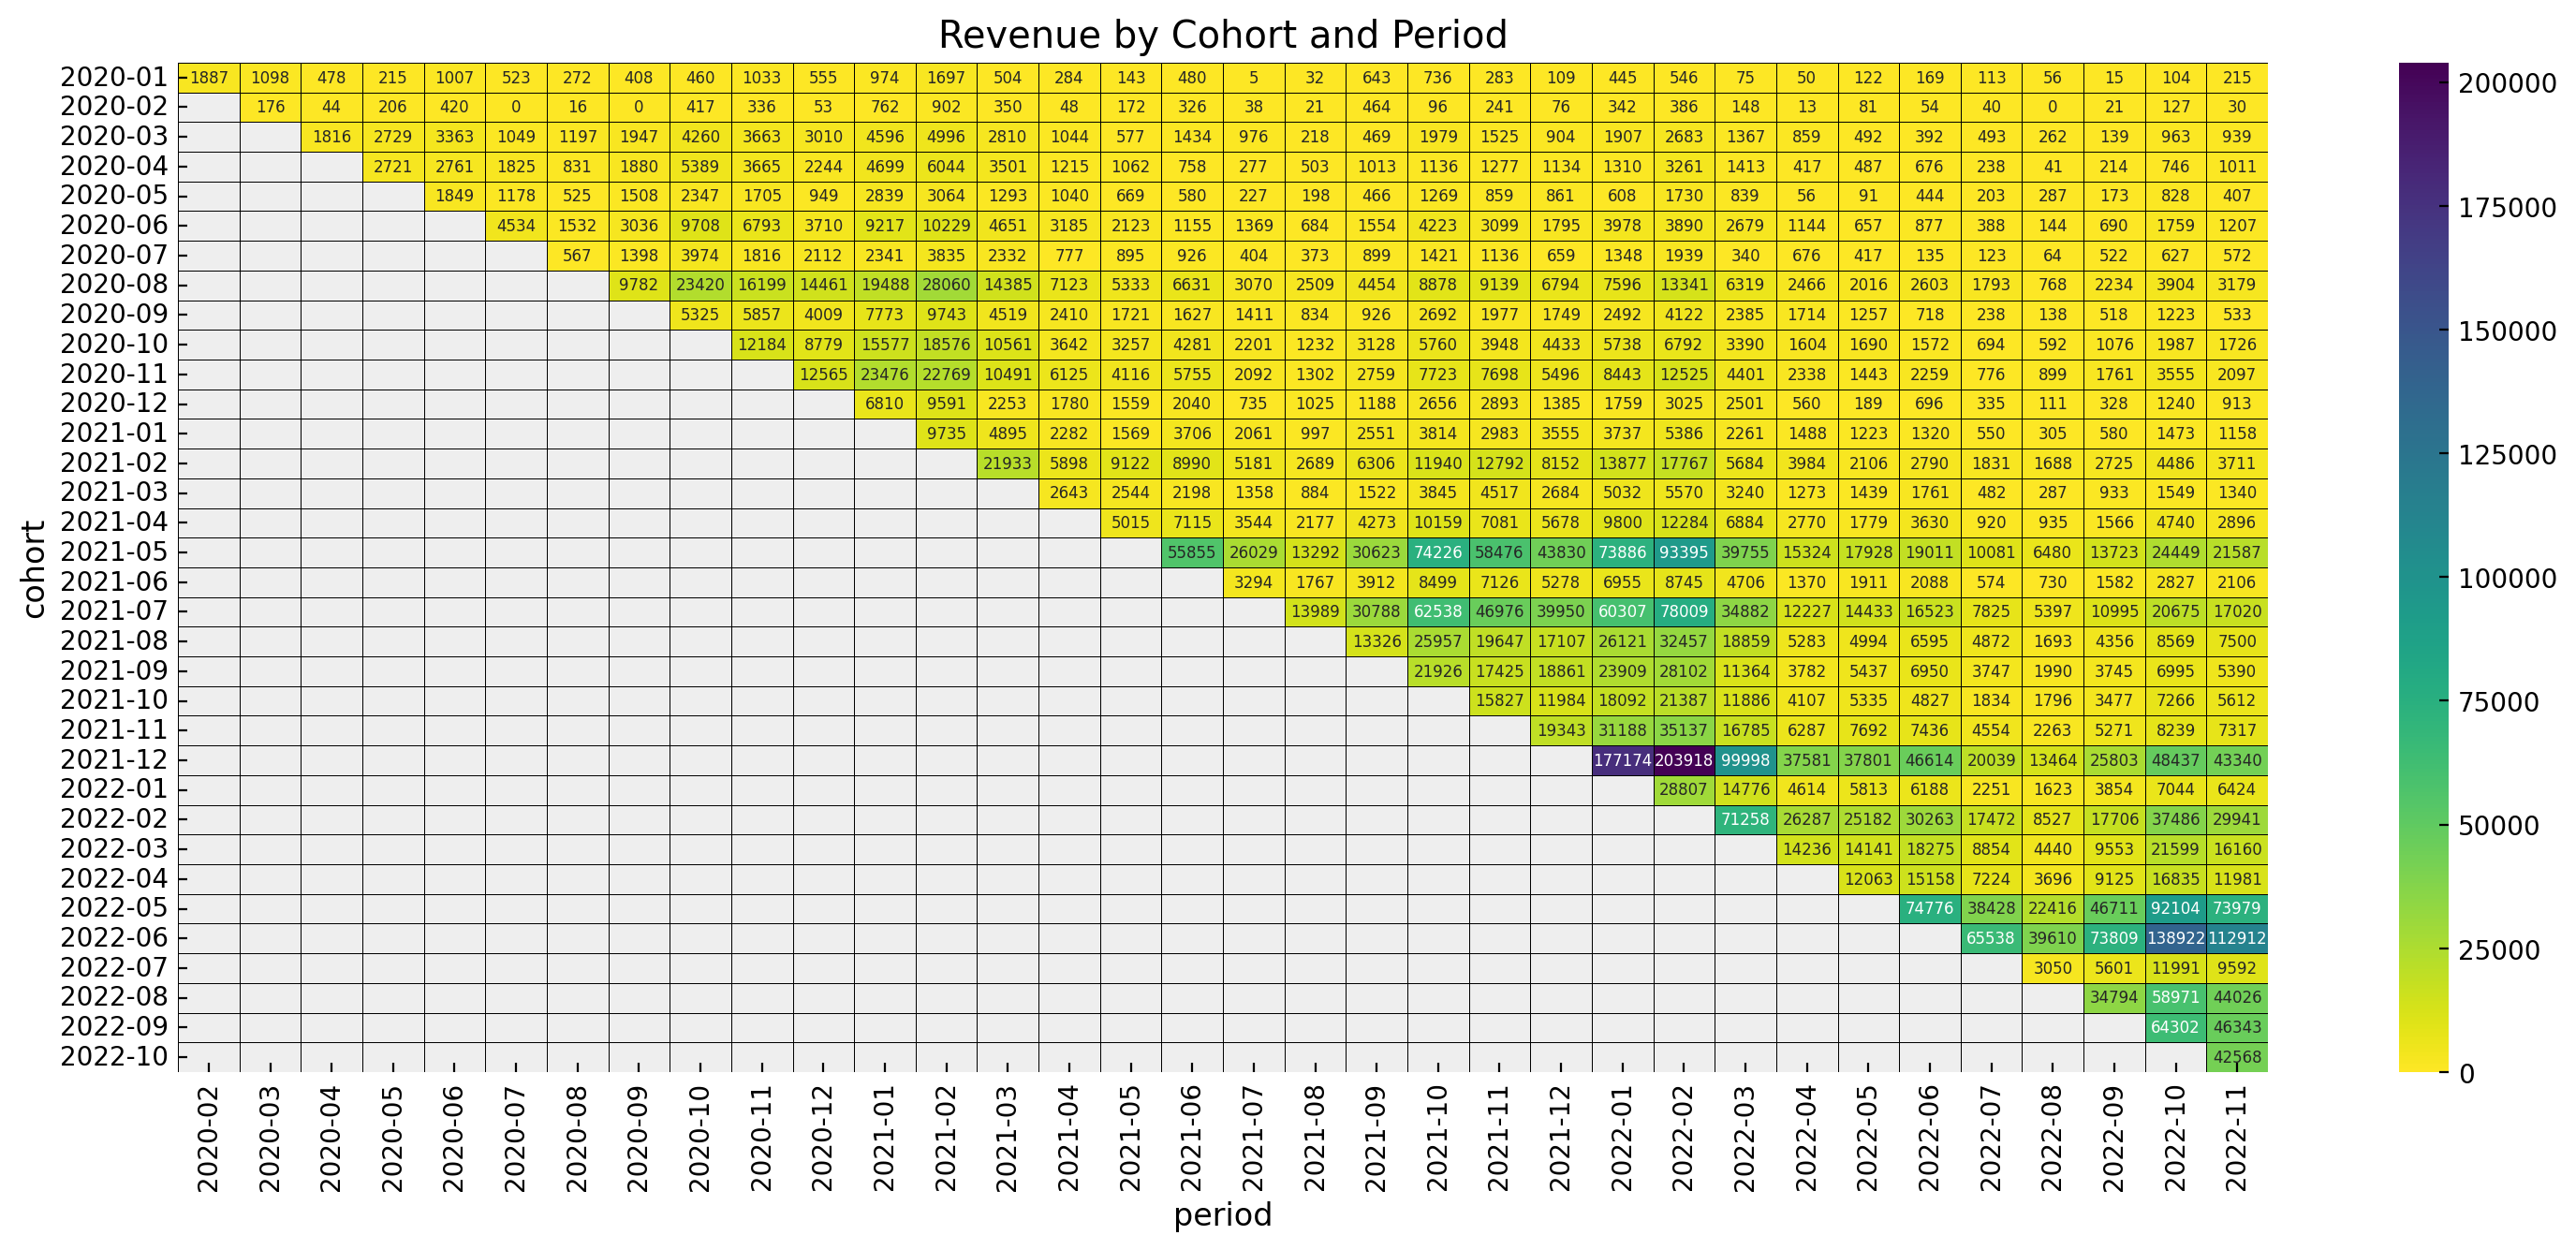
\includegraphics[width=\textwidth]{images/revenue_retention_23_0.png}
    \caption{Revenue per cohort.}
    \label{fig:revenue}
\end{figure}

Now, let us look at the revenue. Figure \ref{fig:revenue} shows the revenue per cohort. 
We see from the plots how the revenue correlates with the number of active users. This 
hints that the revenue per user does not change dramatically over time. To see this,
we can compute the revenue per user as a function of the age and the period (see Figure
\ref{fig:revenue_per_user}). We also can compute the revenue per {\em active} user (see
Figure \ref{fig:revenue_per_active_user}). The main difference between the two is that
for the former we divide by the cohort size, while for the latter we divide by the
number of active users in the given period. Here are some observations:

\begin{itemize}
    \item The revenue per user shows a clear seasonality pattern. This is expected as
        the retention has a seasonality pattern.
    \item The revenue per active user does now the seasonality pattern as it s already
        encoded in the denominator. In addition, we see that the revenue per active user
        seems to be decreasing as the cohort age increases.
\end{itemize}

\begin{figure}
    \centering
    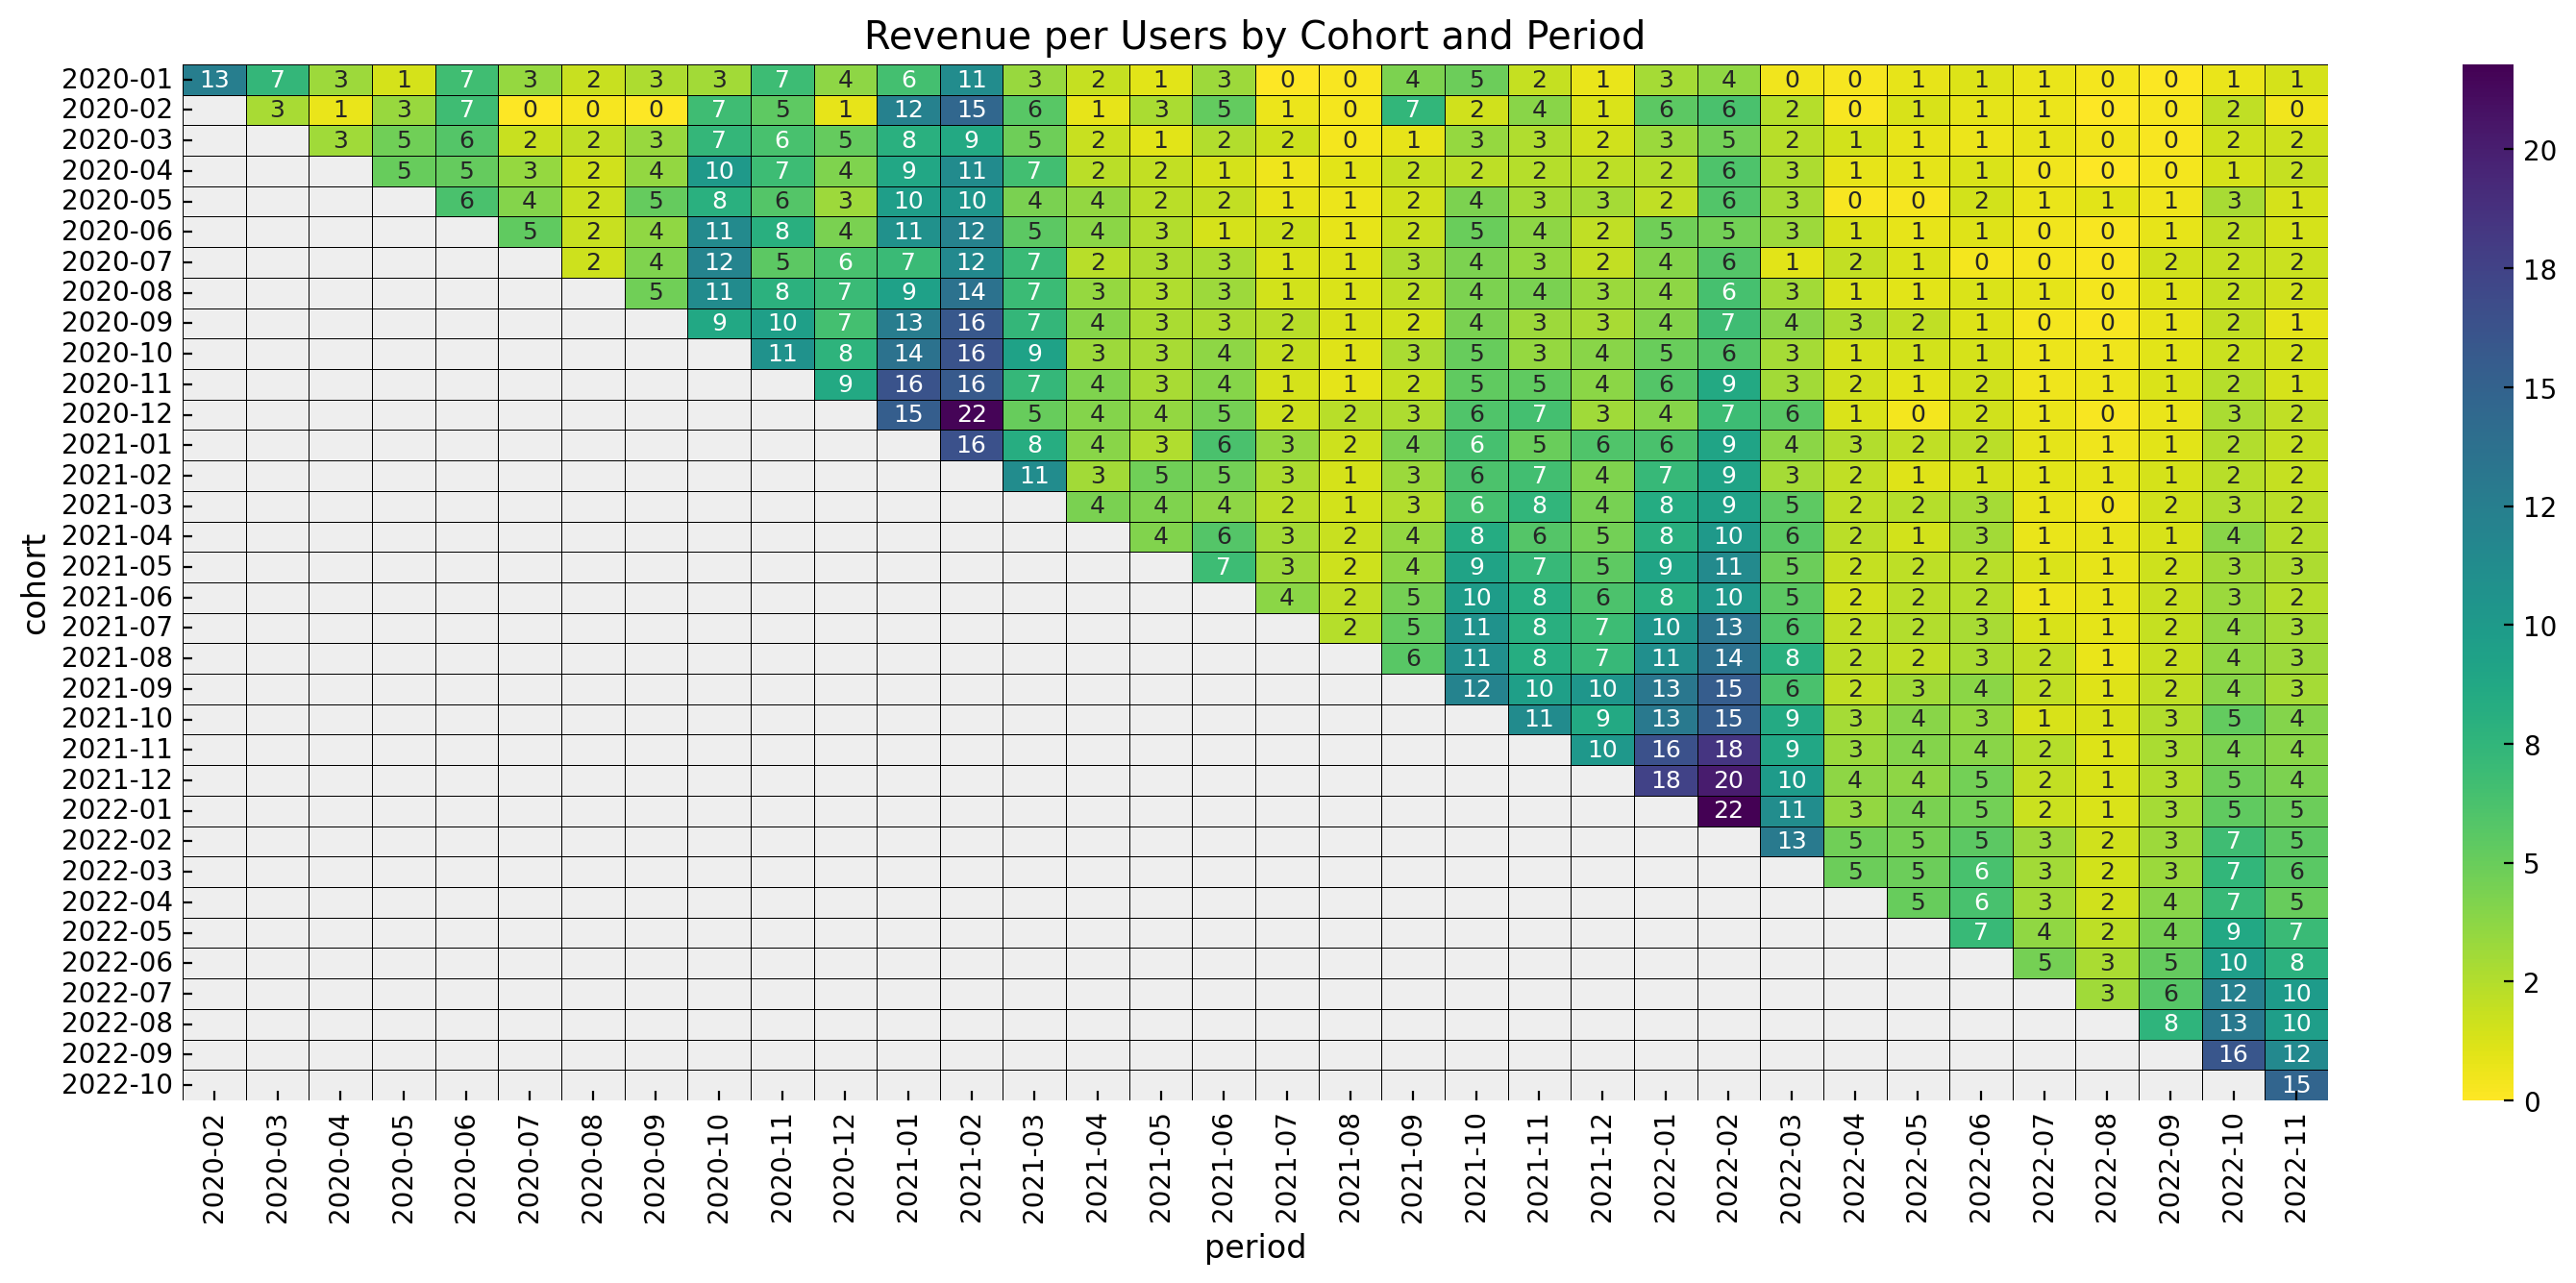
\includegraphics[width=\textwidth]{images/revenue_retention_27_0.png}
    \caption{Revenue per cohort.}
    \label{fig:revenue_per_user}
\end{figure}

\begin{figure}
    \centering
    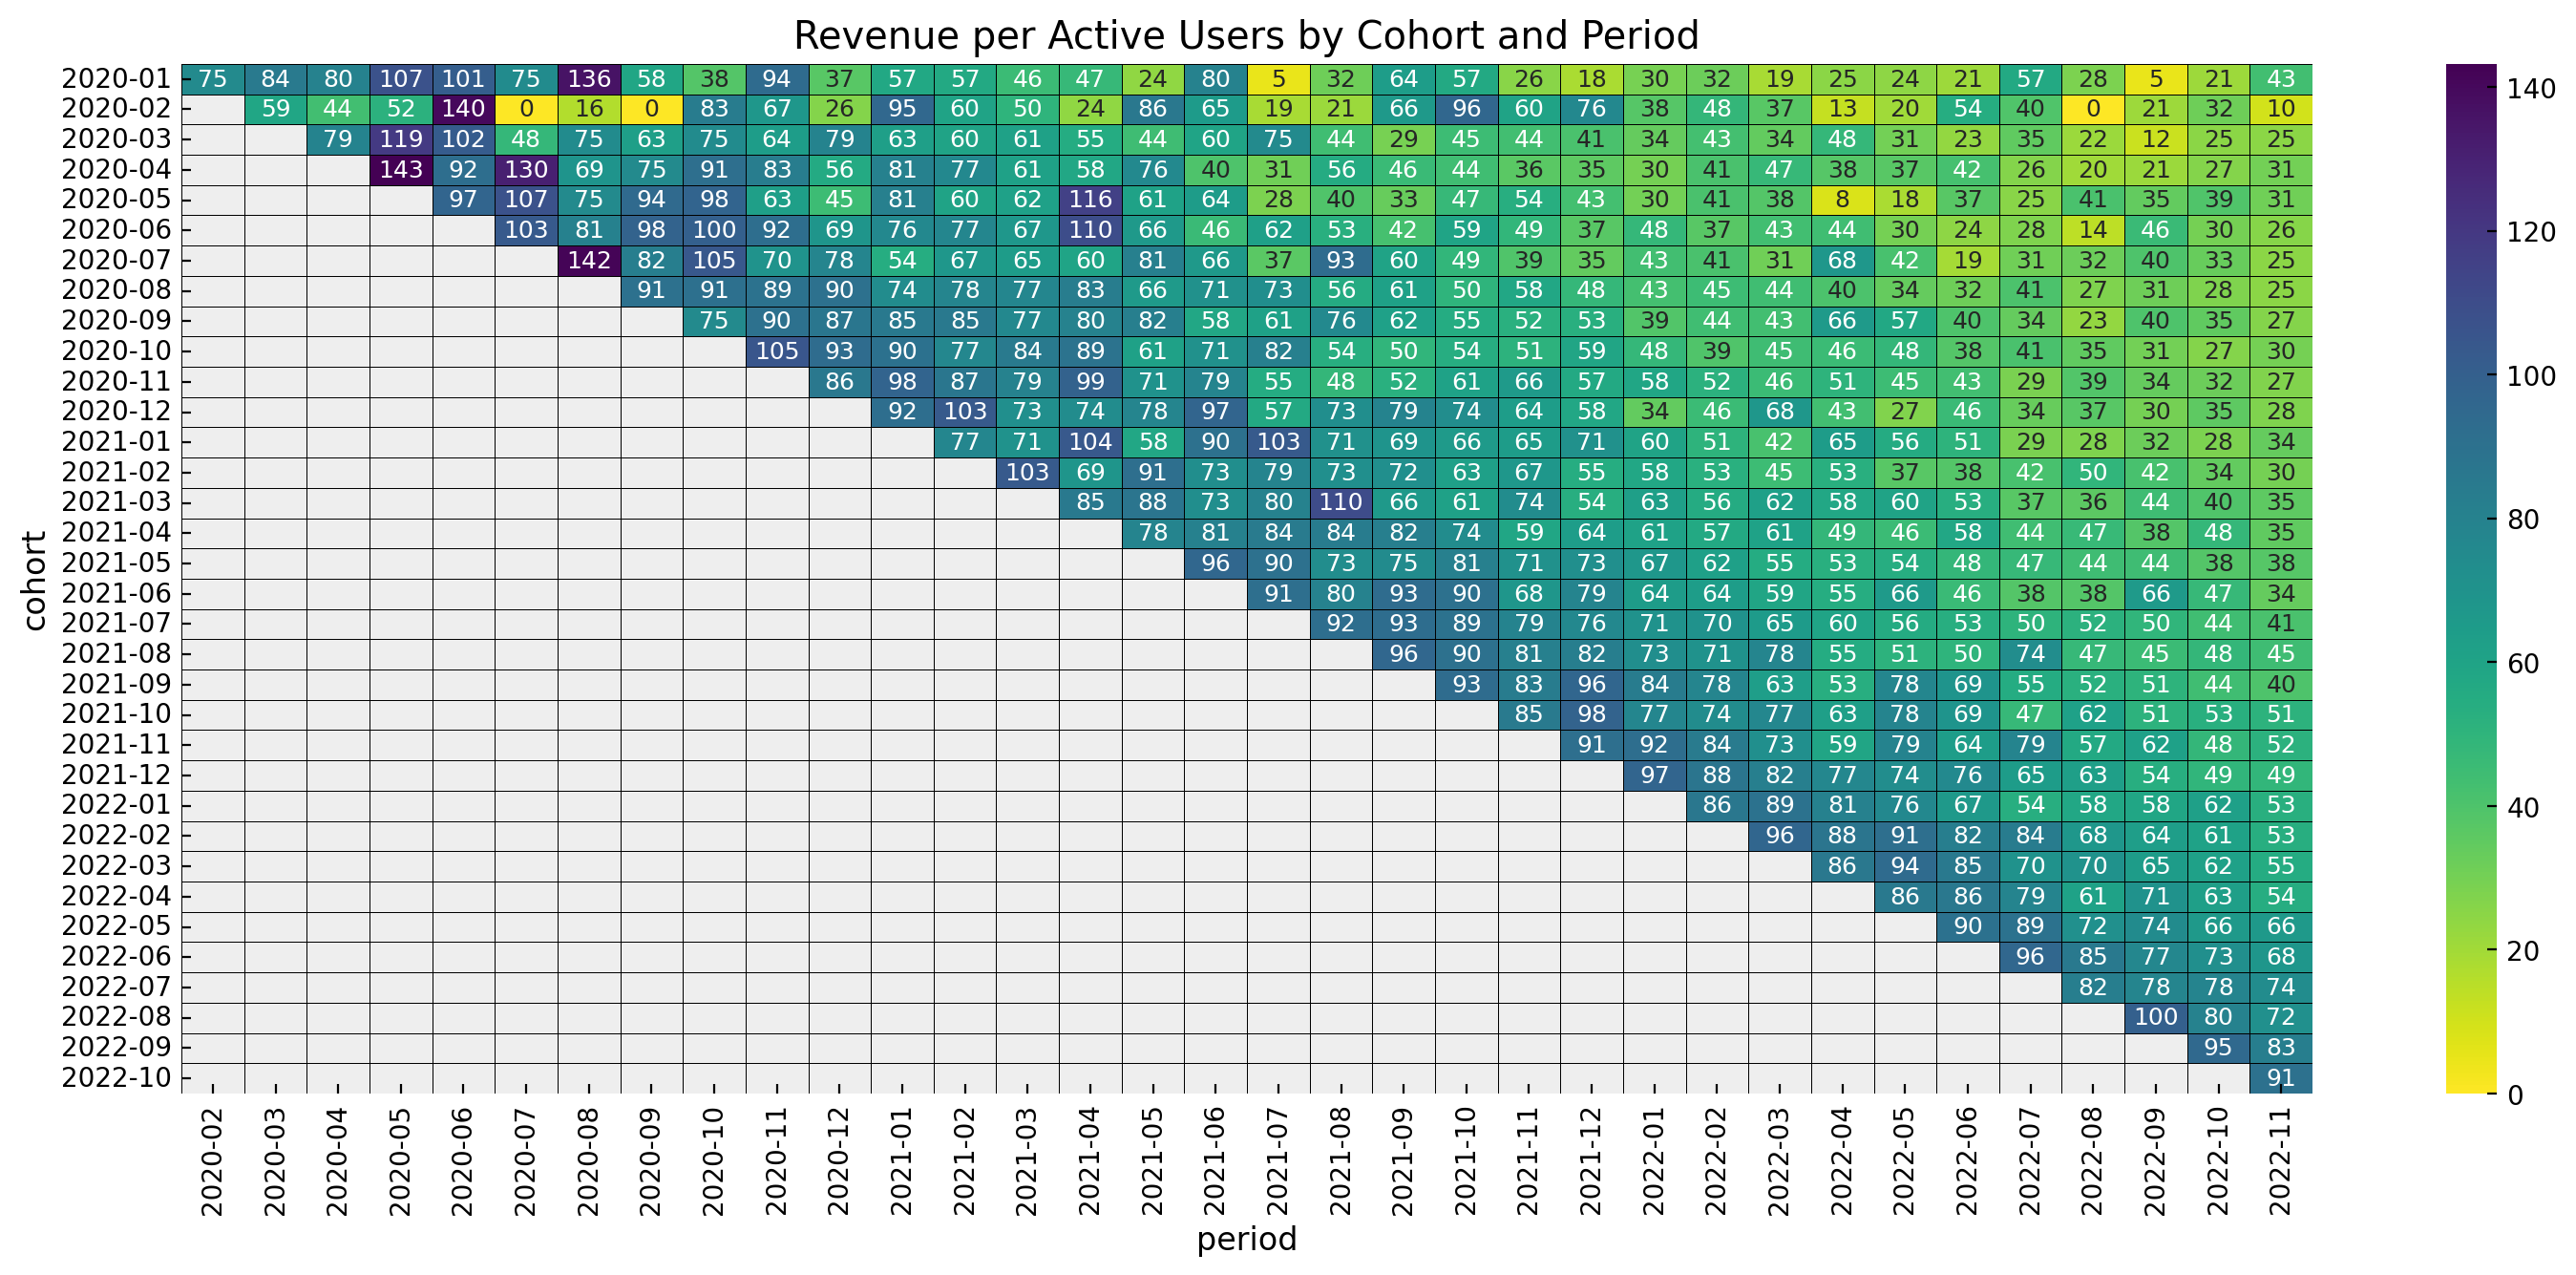
\includegraphics[width=\textwidth]{images/revenue_retention_25_0.png}
    \caption{Revenue per cohort.}
    \label{fig:revenue_per_active_user}
\end{figure}

After this exploratory analysis, we can start the modeling phase.

\section{Model Specification and Diagnostics}

Now we expand on the model structure described in the introduction. The main idea is to
model the number of active users as a binomial random variable
$\text{Binomial}(N_{\text{total}}, p)$, where the parameter $p$ represents the retention.
We use bayesian additive regression trees (BART) to model the latent variable $p$ using
as features cohort age, age and (period) month. One could of course start with a simpler
model, say a linear model as described in \cite{orduz_revenue_retention}. Nevertheless,
in real datasets, this approach does not fit the data well. \\

On the other hand, we model the revenue as a gamma random variable
$\text{Gamma}(N_{\text{active}}, \lambda)$, where the parameter $\lambda$ is modeled
through a linear model of the cohort age and age (and potentially higher-order
interactions). One of the key observations we have seen in many real applications (and 
also in this synthetic data set is that we do not need to add a seasonality component
into the retention model as it is already captured by the retention itself.

\begin{figure}
    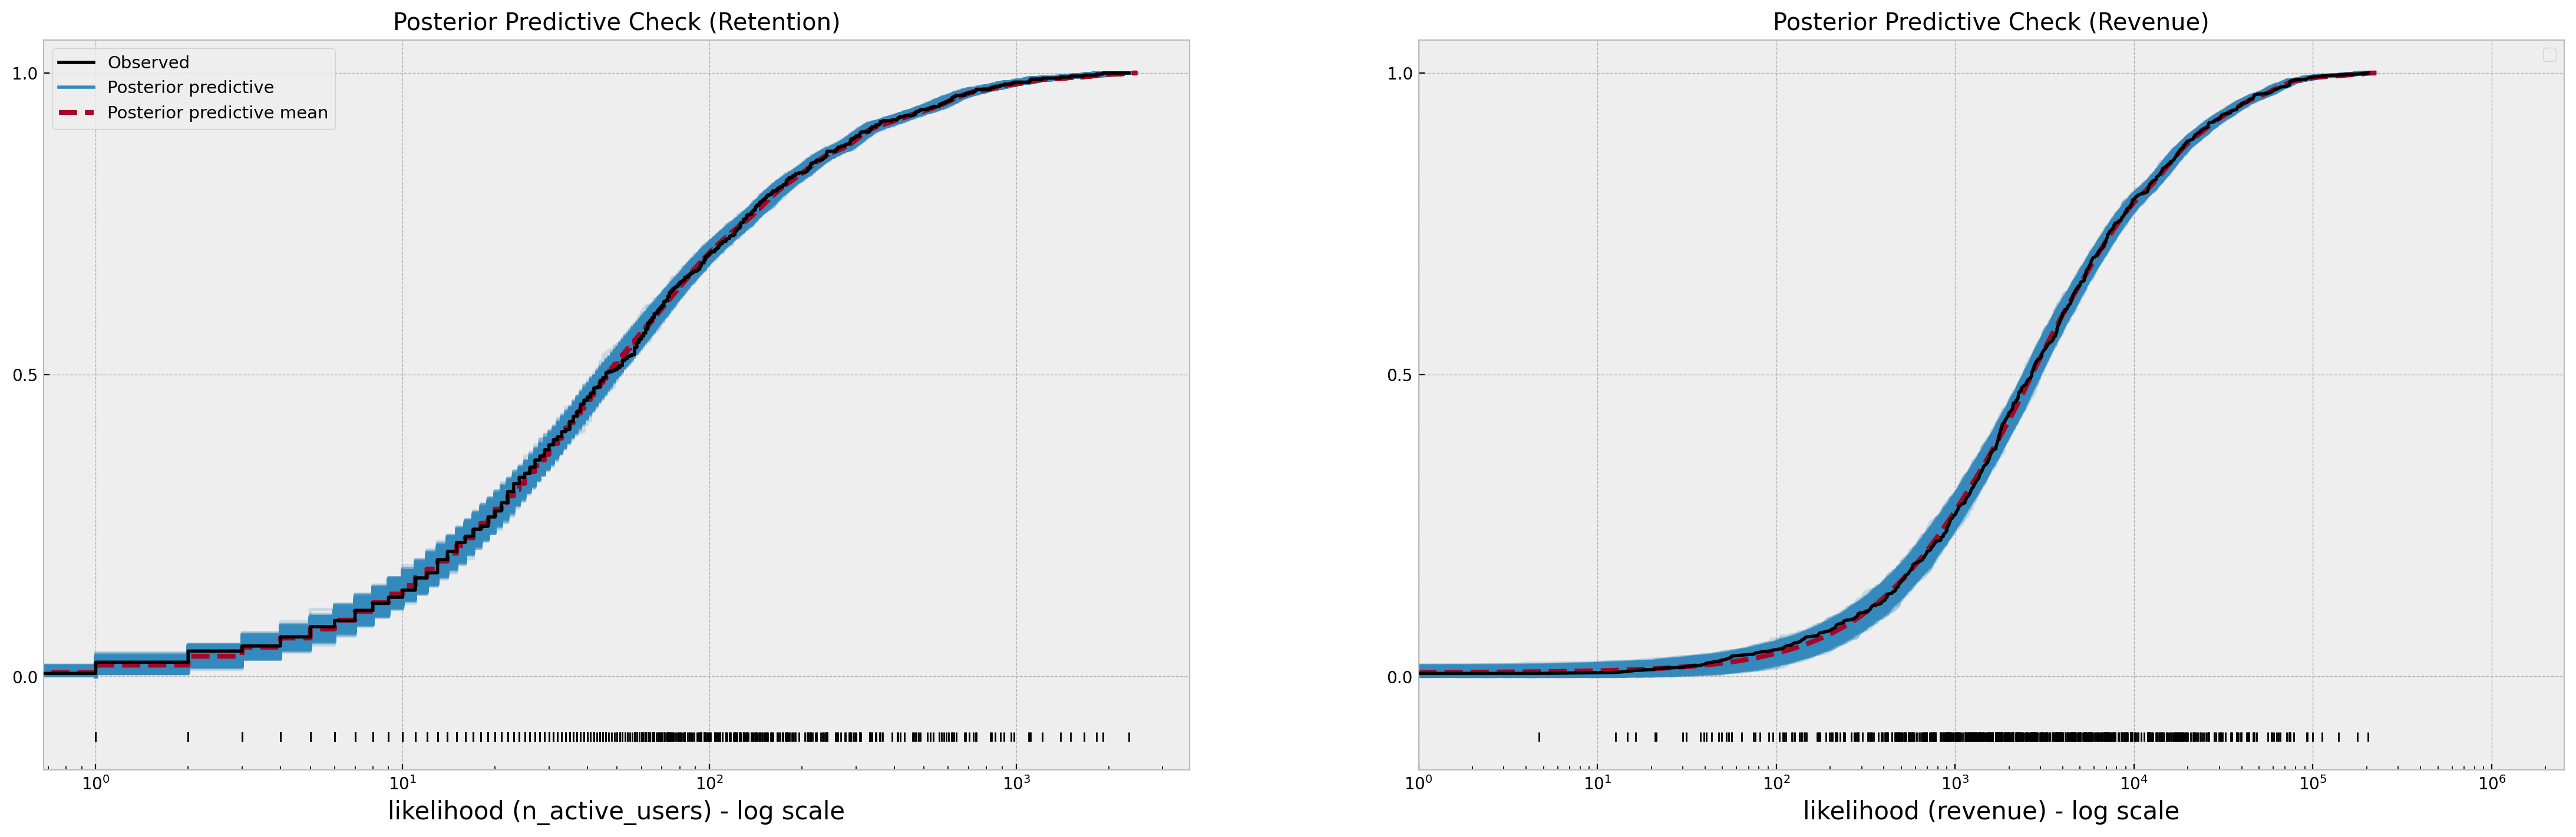
\includegraphics[width=\textwidth]{images/revenue_retention_37_0.png}
\end{figure}

\begin{figure}
    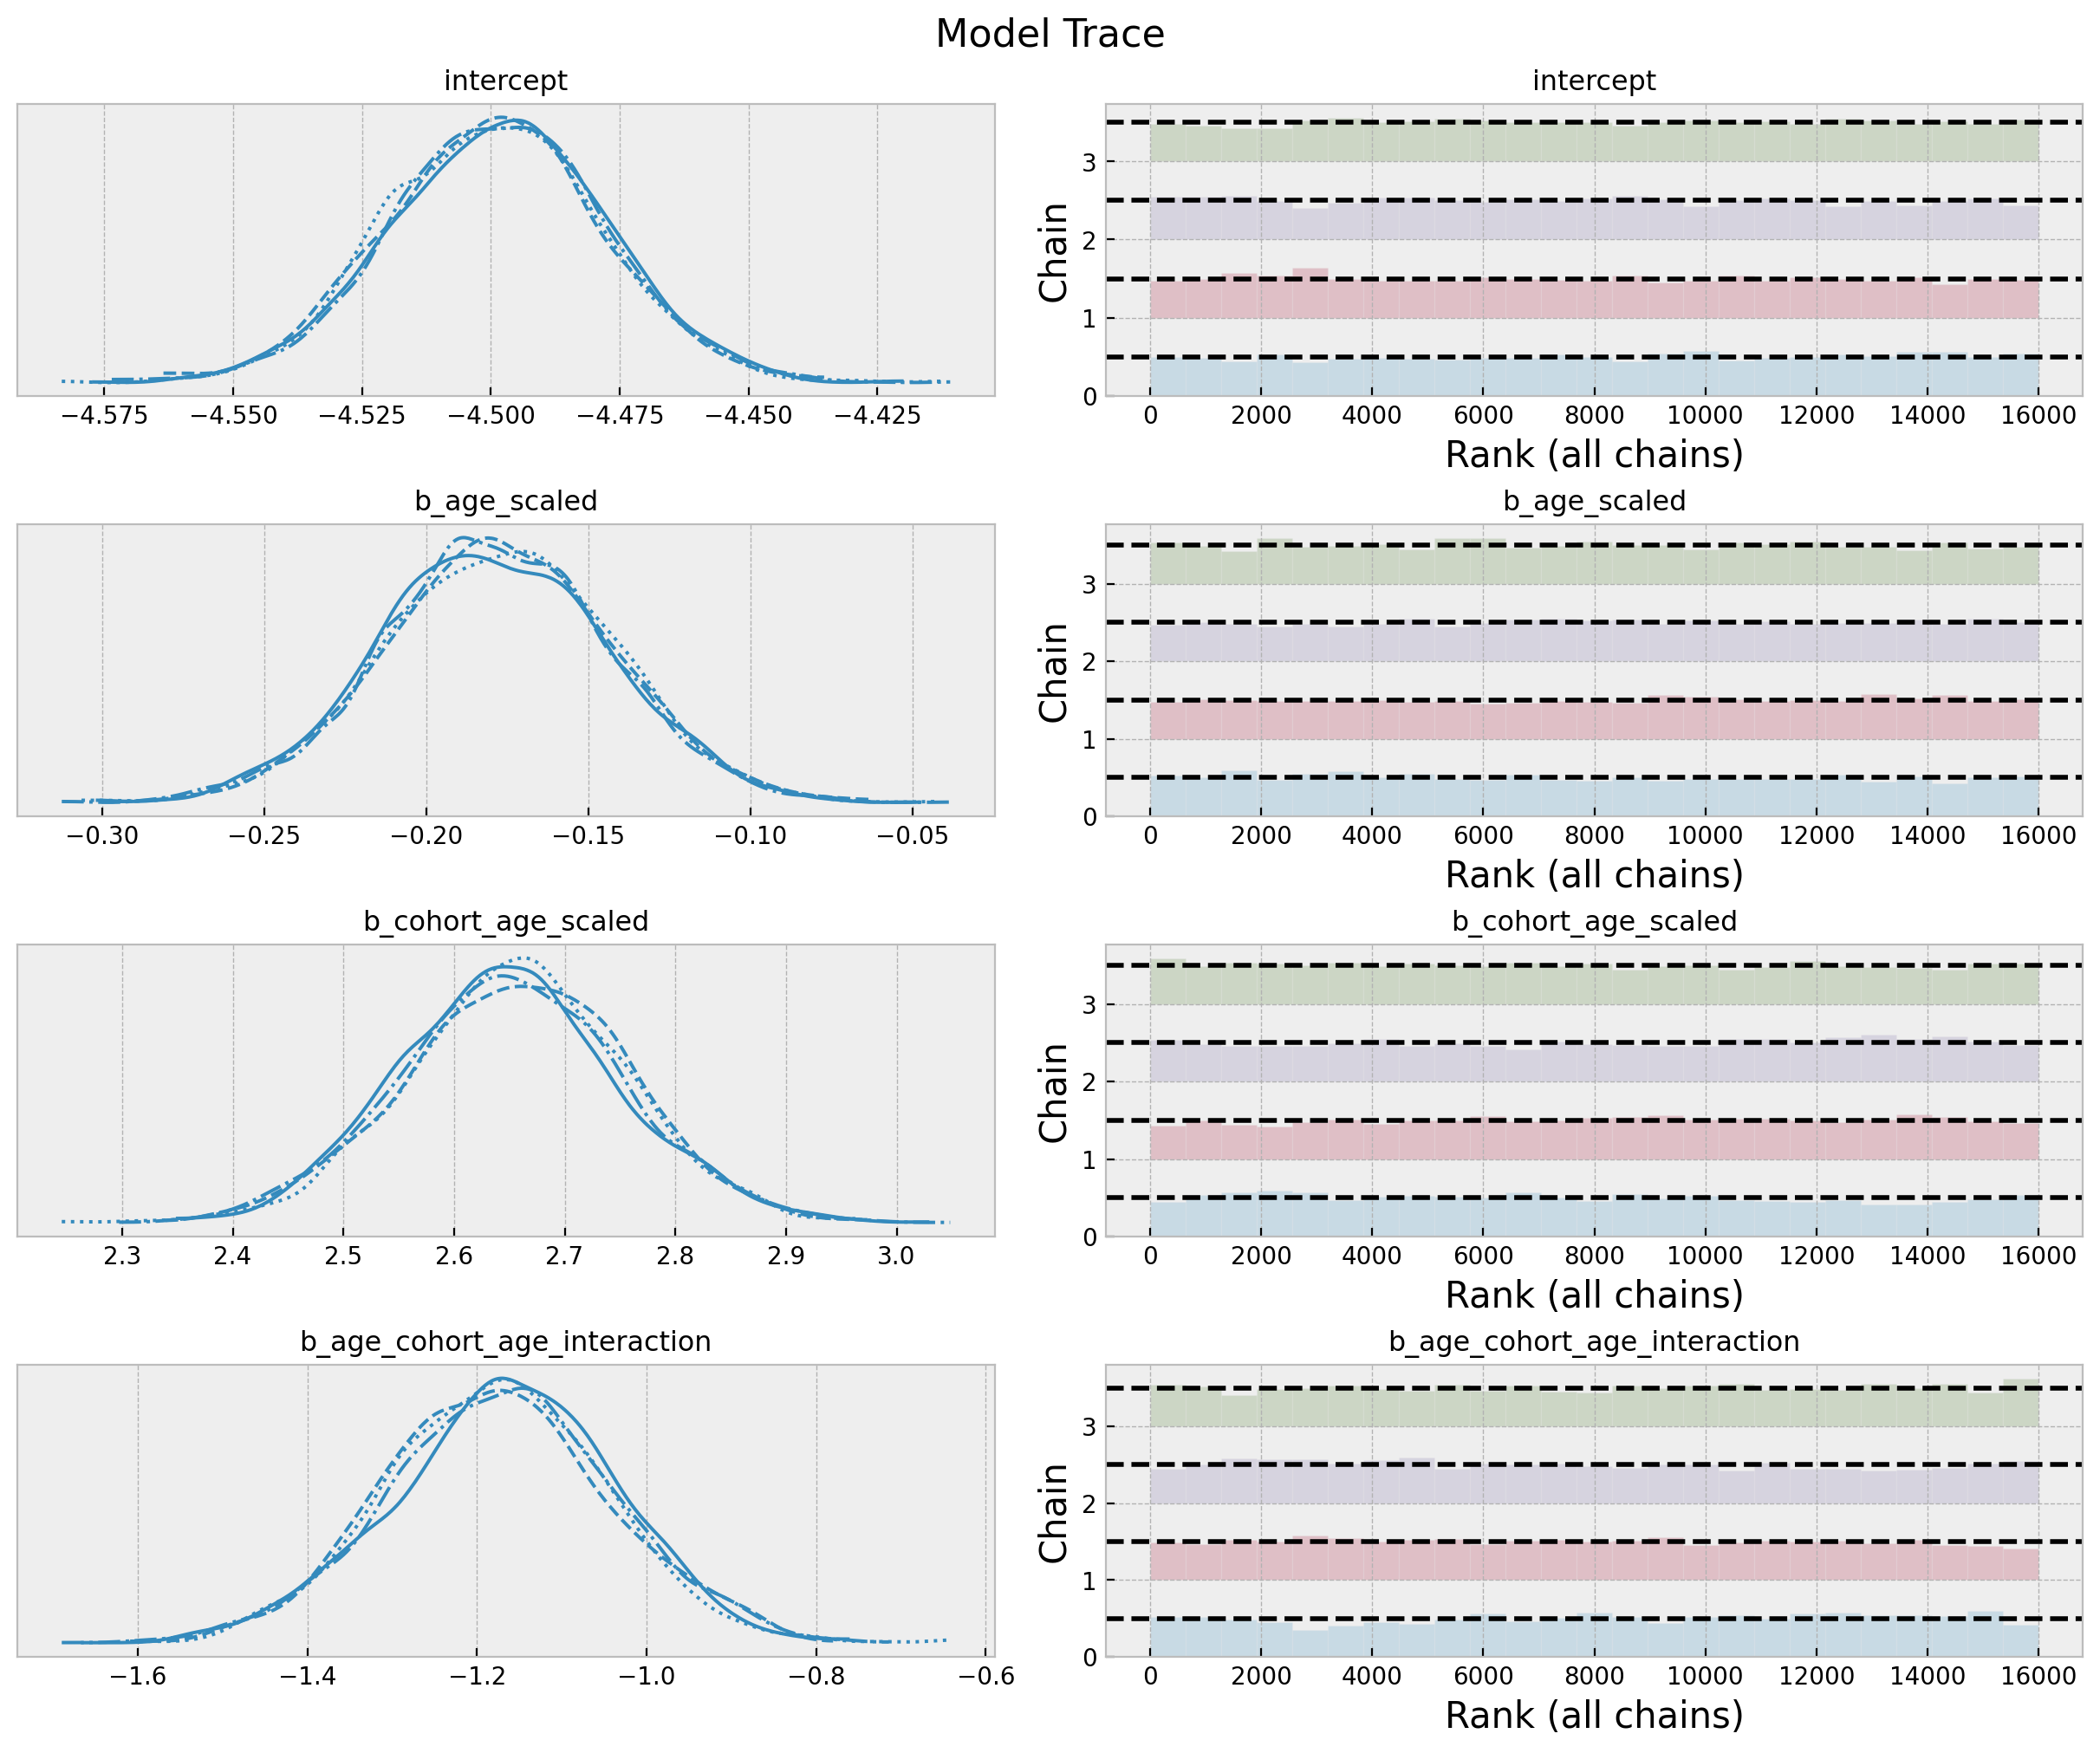
\includegraphics[width=\textwidth]{images/revenue_retention_41_0.png}
\end{figure}

\section{Predictions}

\subsection{In-Sample Predictions}

\begin{figure}
    \begin{tabular}{cc}
        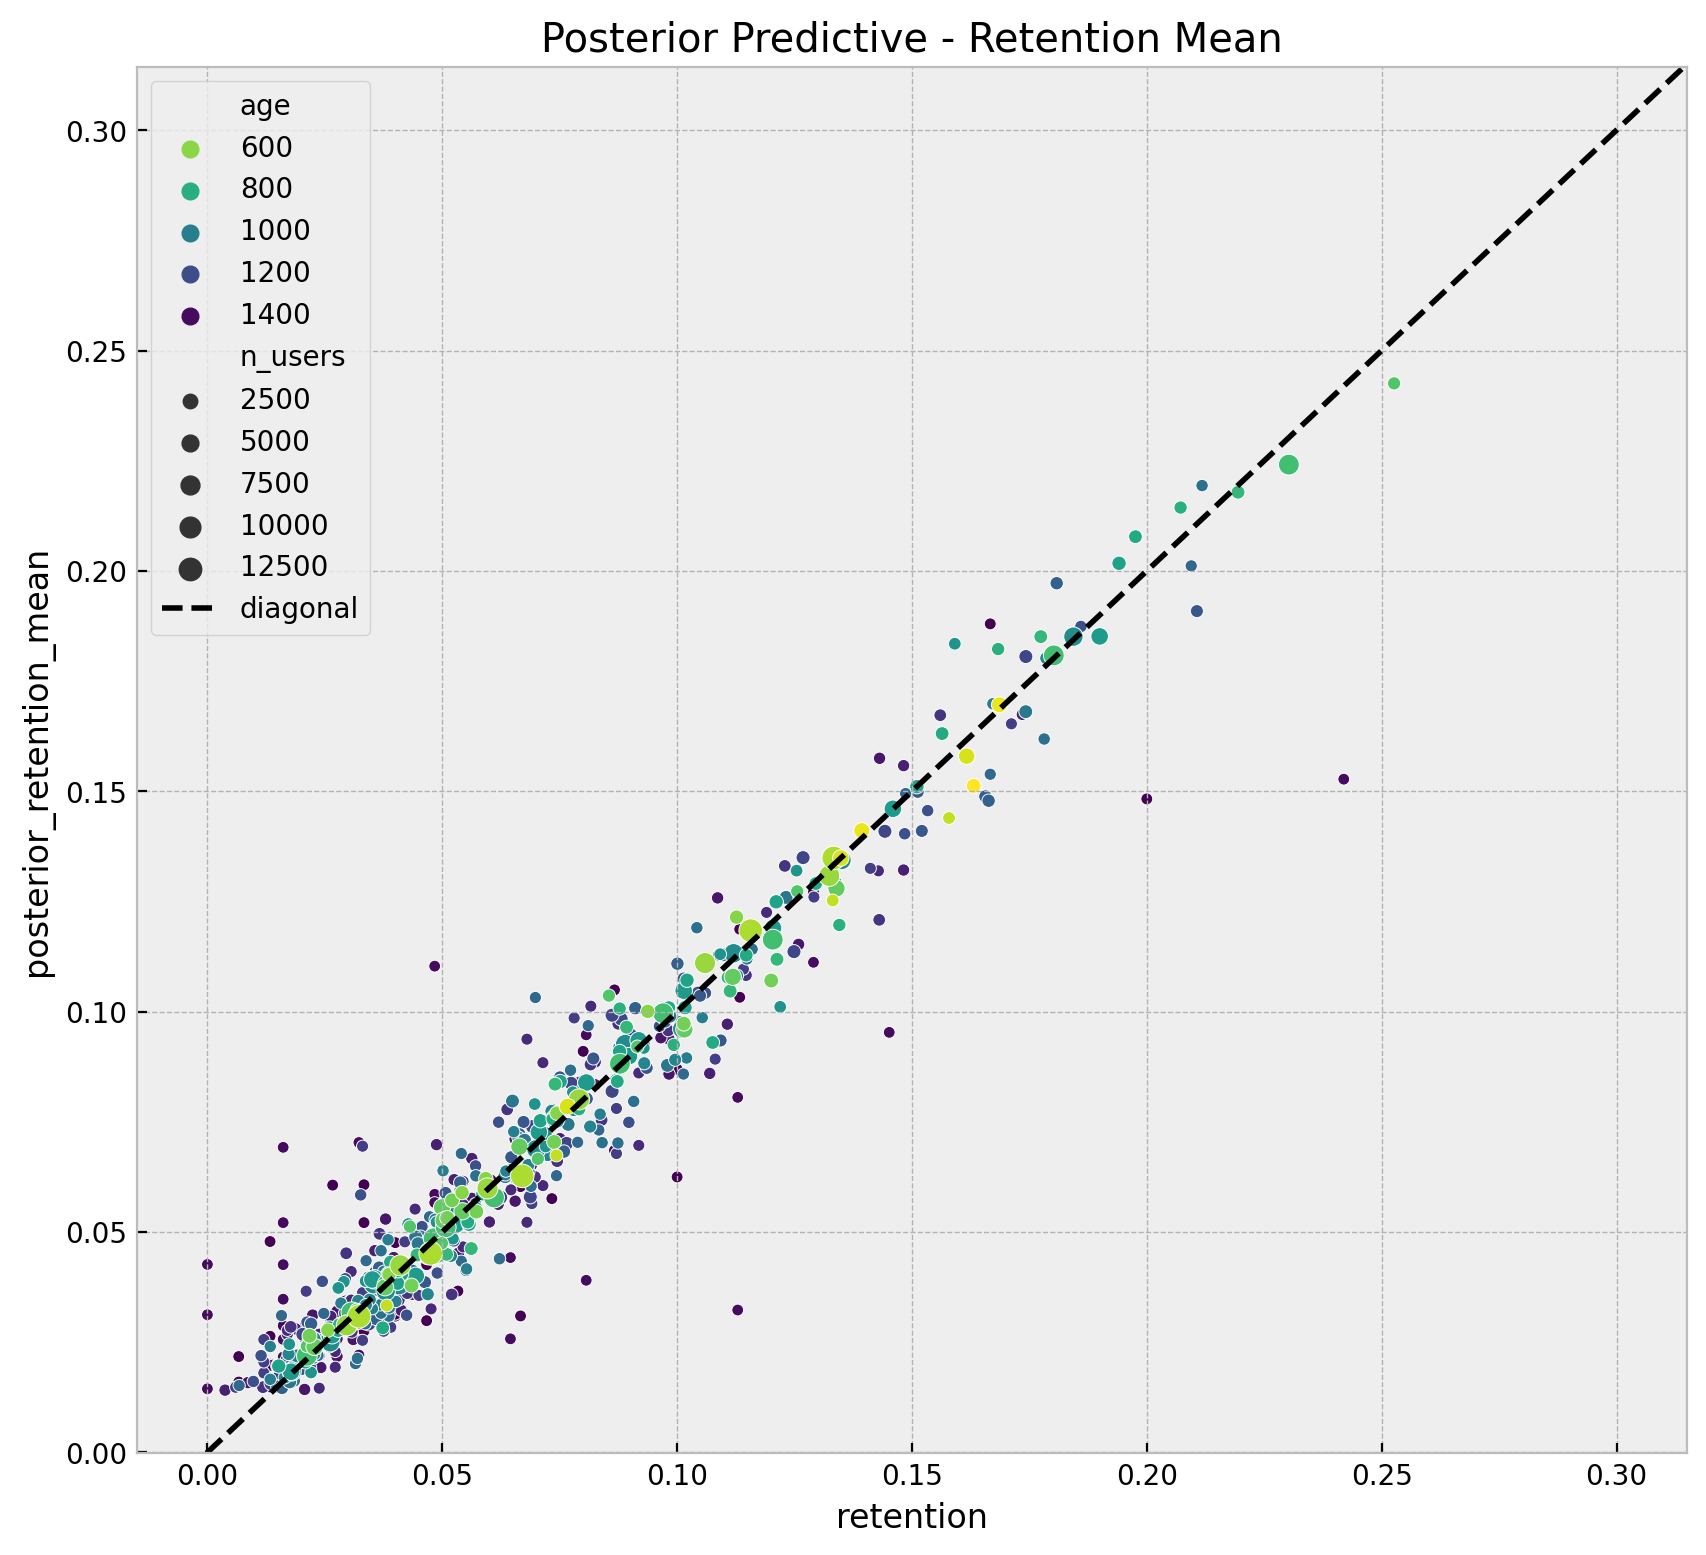
\includegraphics[width=0.5 \textwidth]{images/revenue_retention_45_0.png} & 
        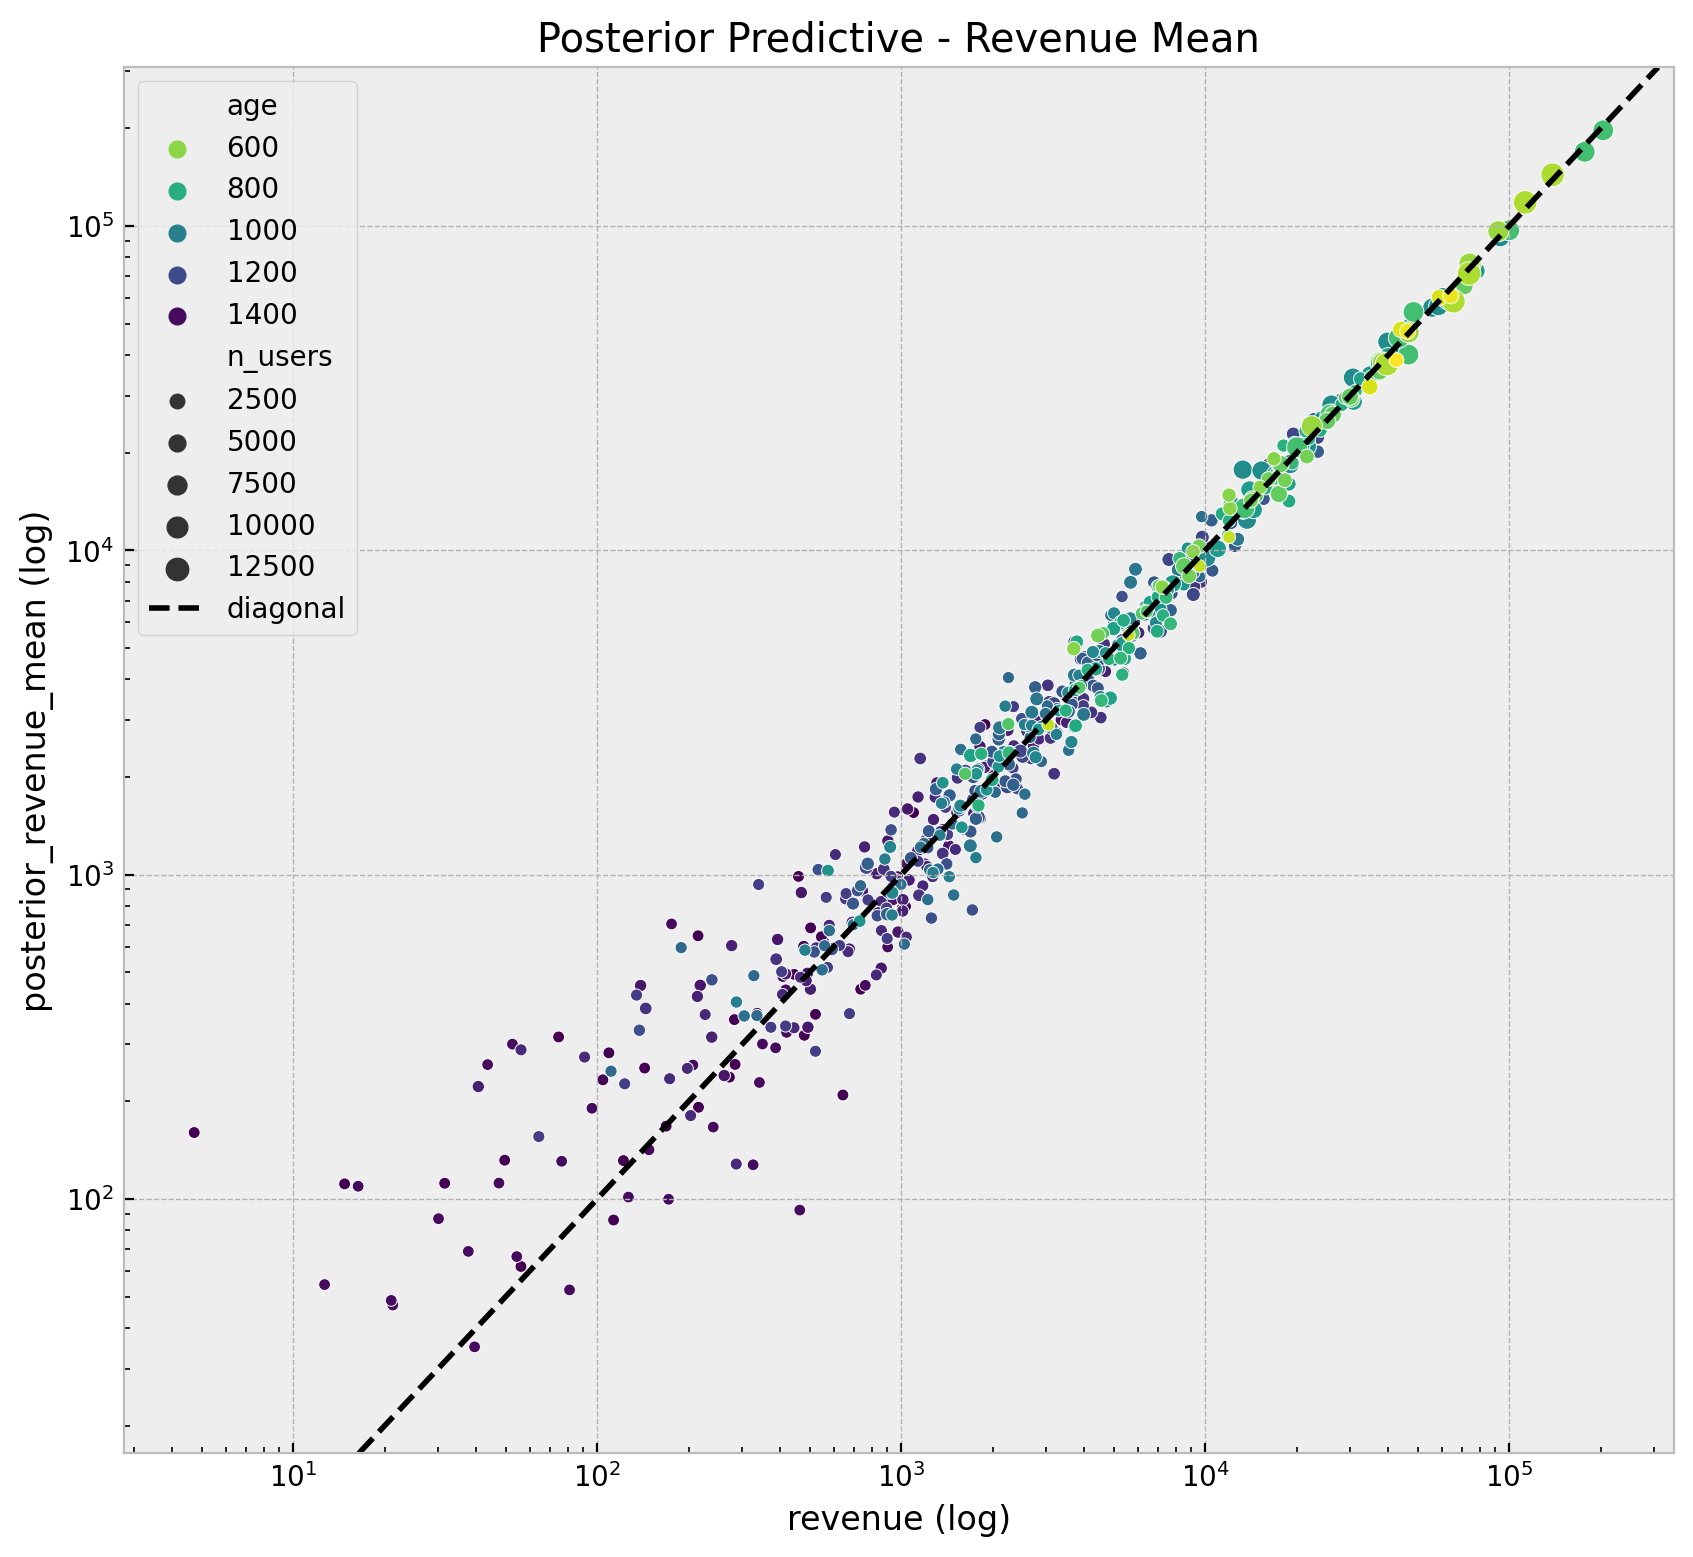
\includegraphics[width=0.5 \textwidth]{images/revenue_retention_47_0.png}
    \end{tabular}
    \caption{My caption}
\end{figure}

\begin{figure}
    \begin{tabular}{cc}
        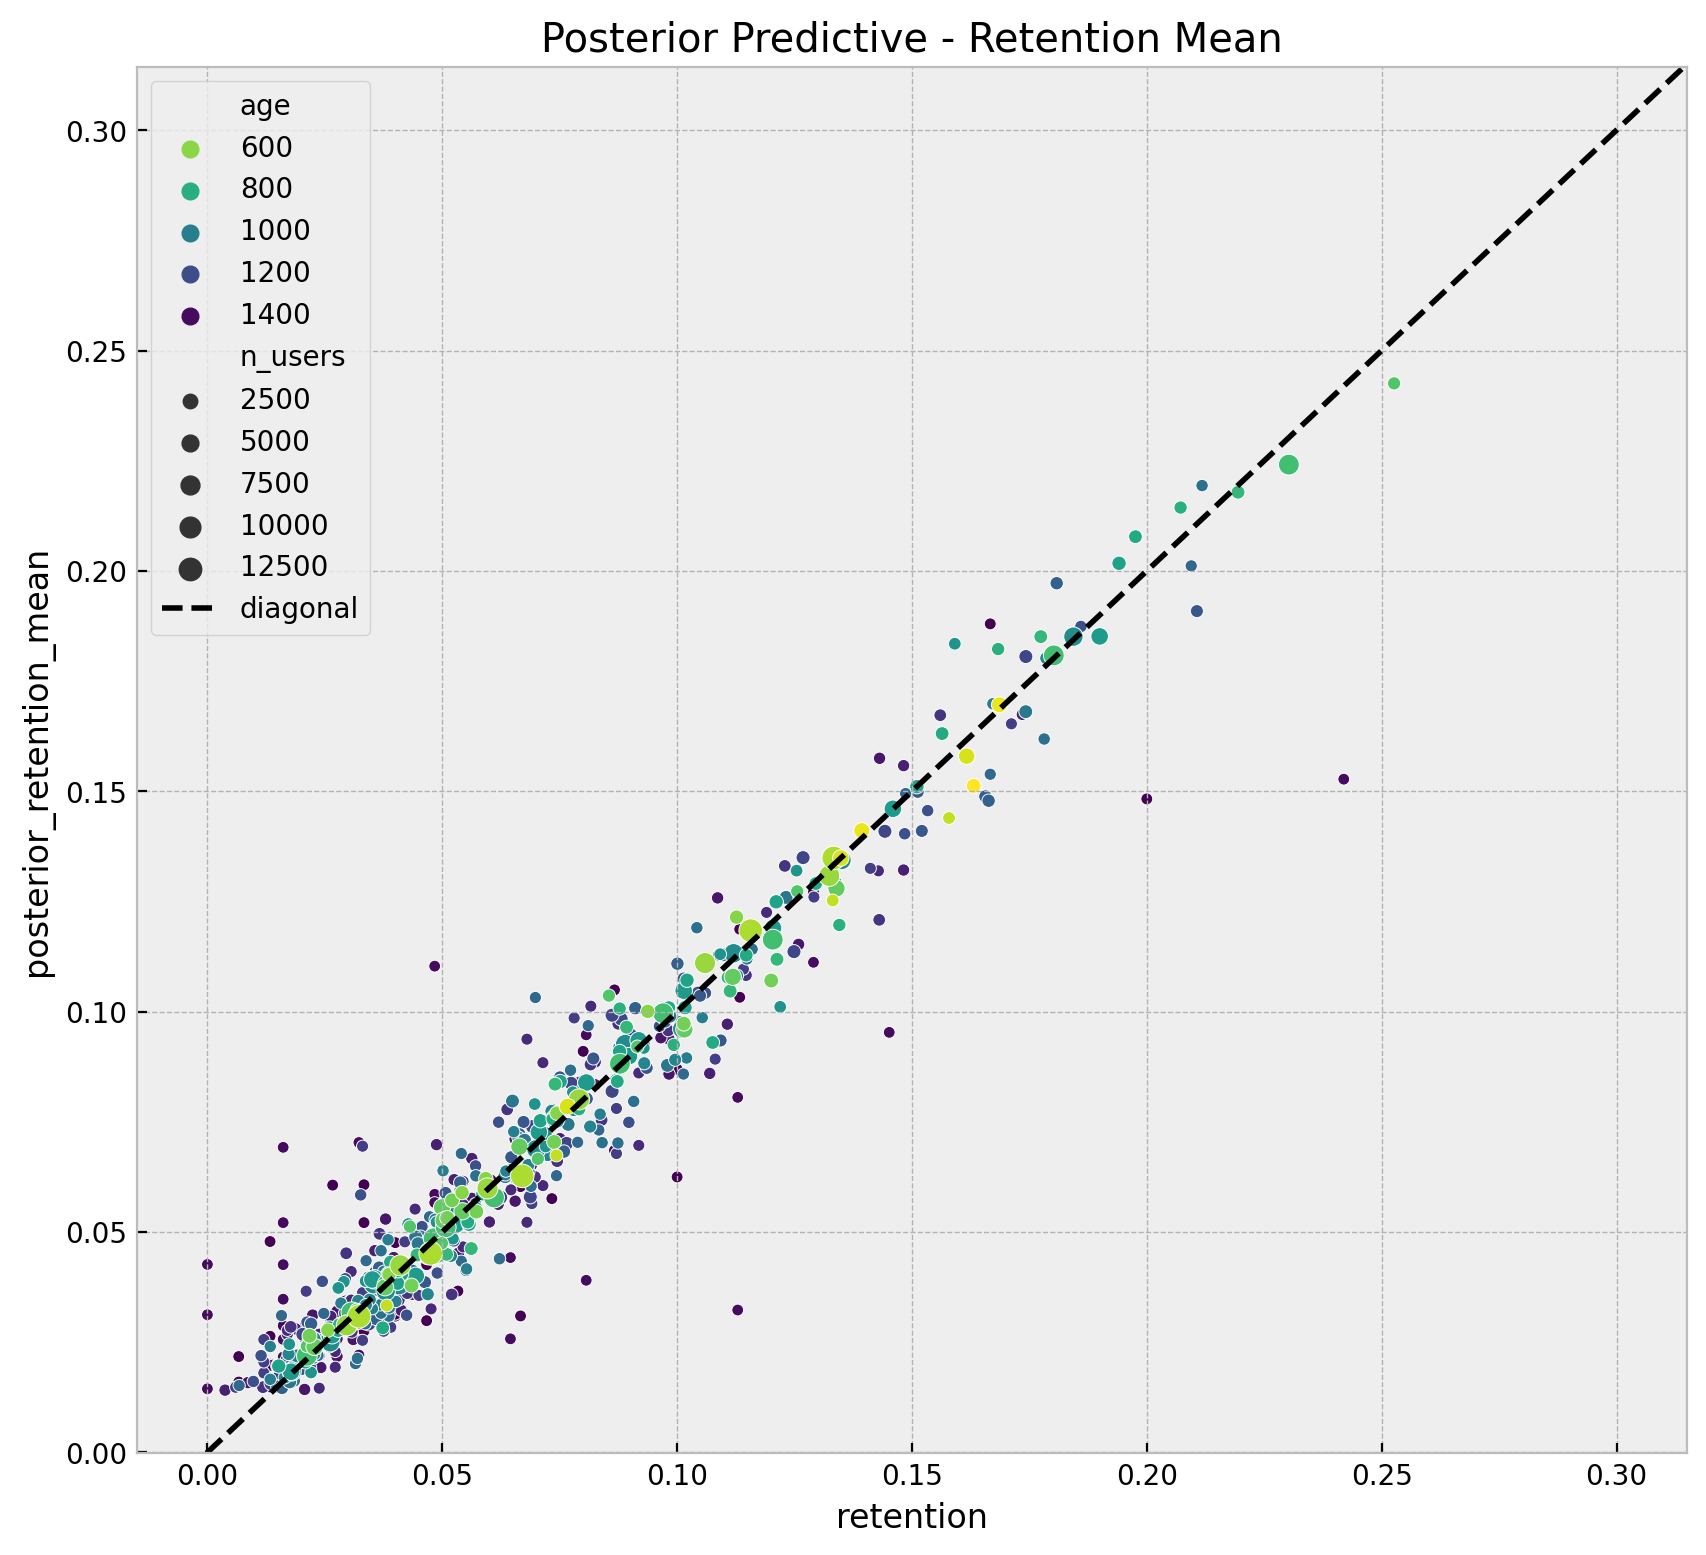
\includegraphics[width=0.5 \textwidth]{images/revenue_retention_45_0.png} & 
        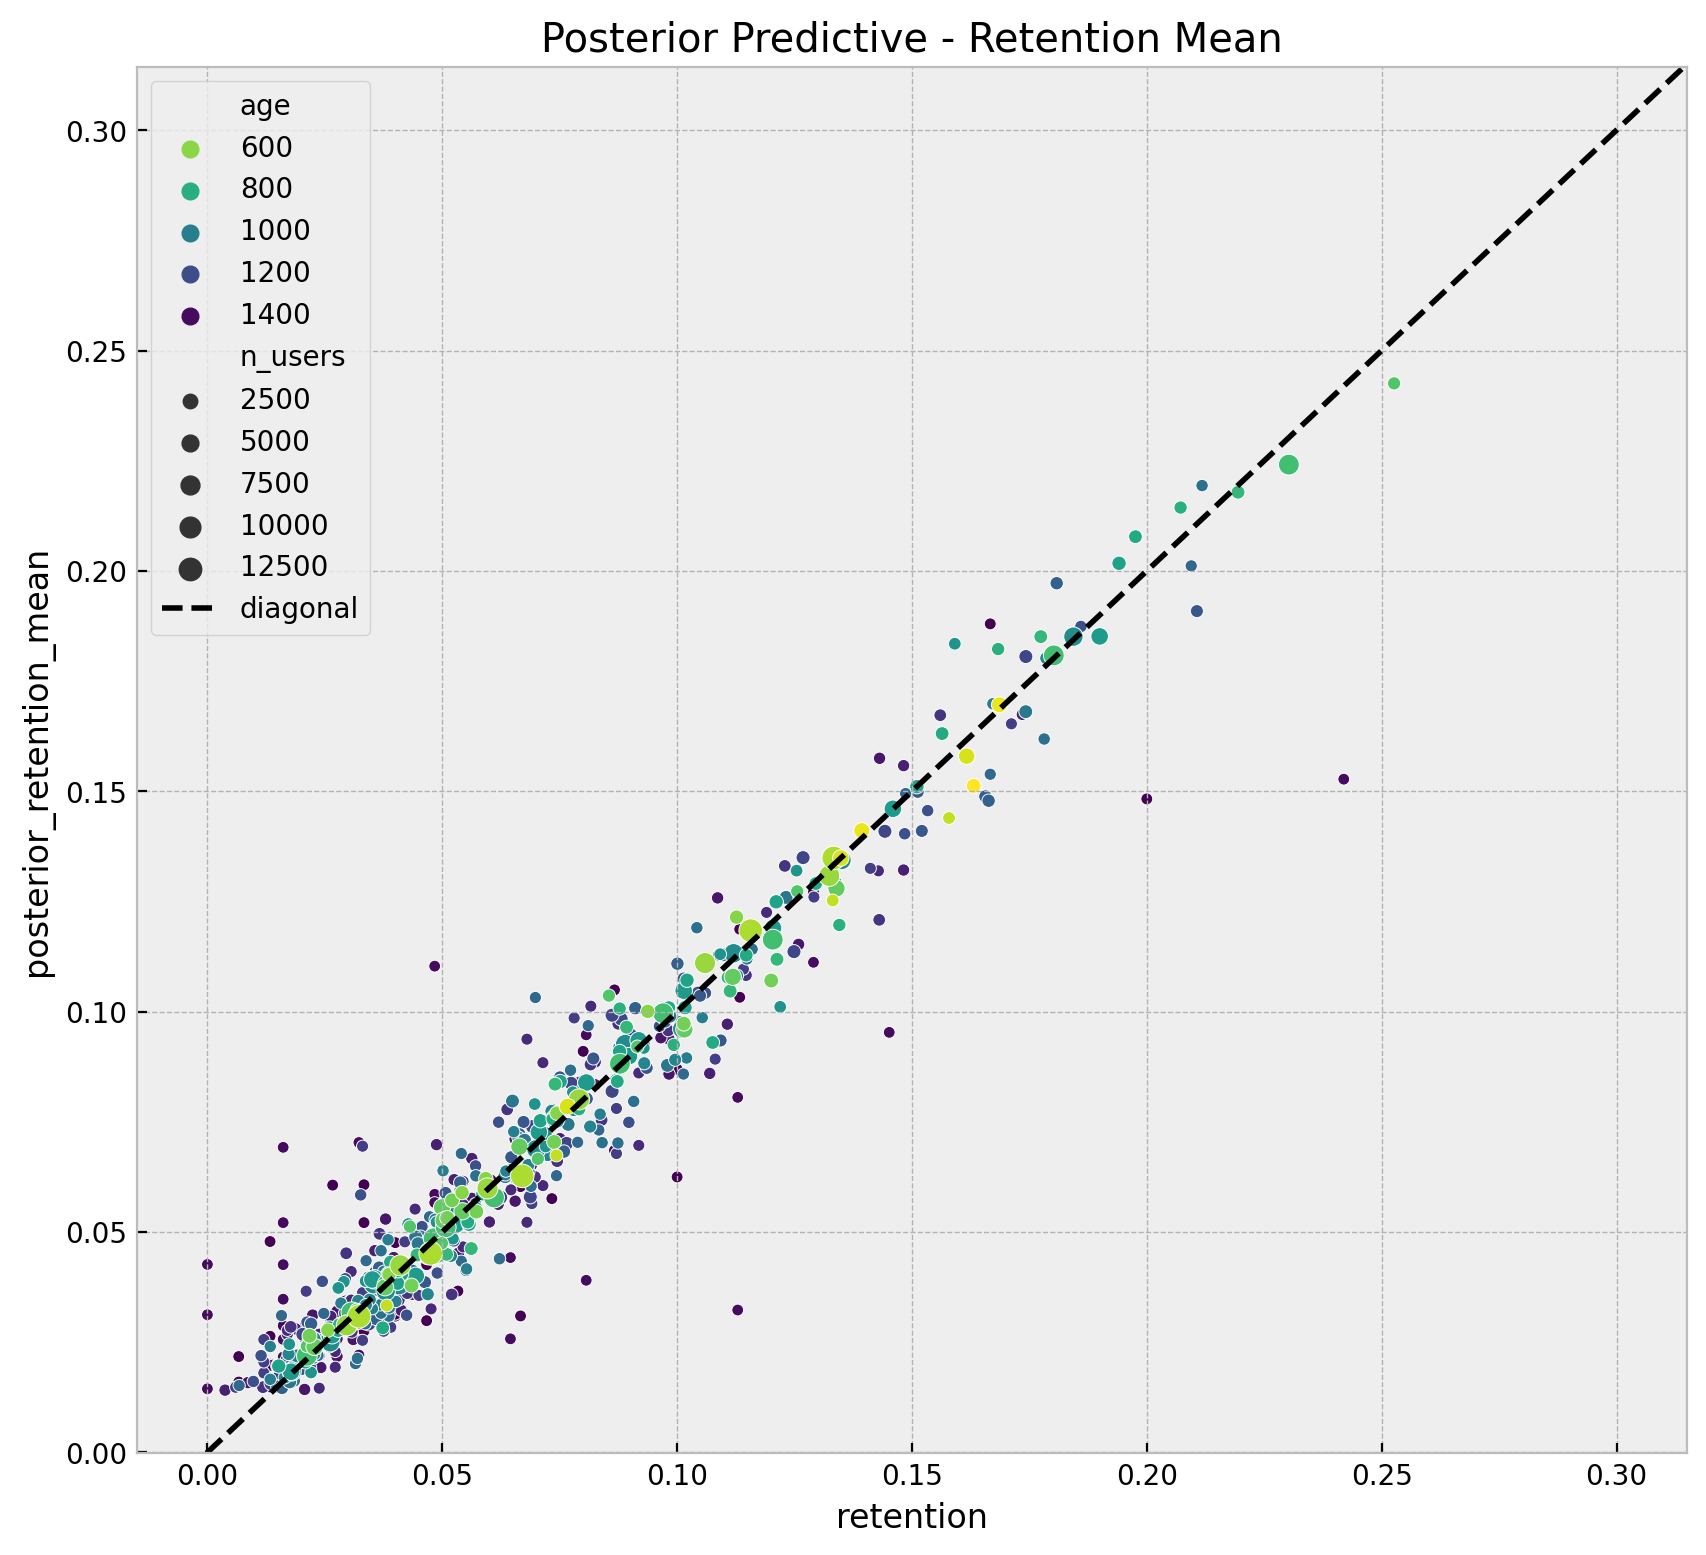
\includegraphics[width=0.5 \textwidth]{images/revenue_retention_45_0.png}
    \end{tabular}
    \caption{My caption}
\end{figure}

\begin{figure}
    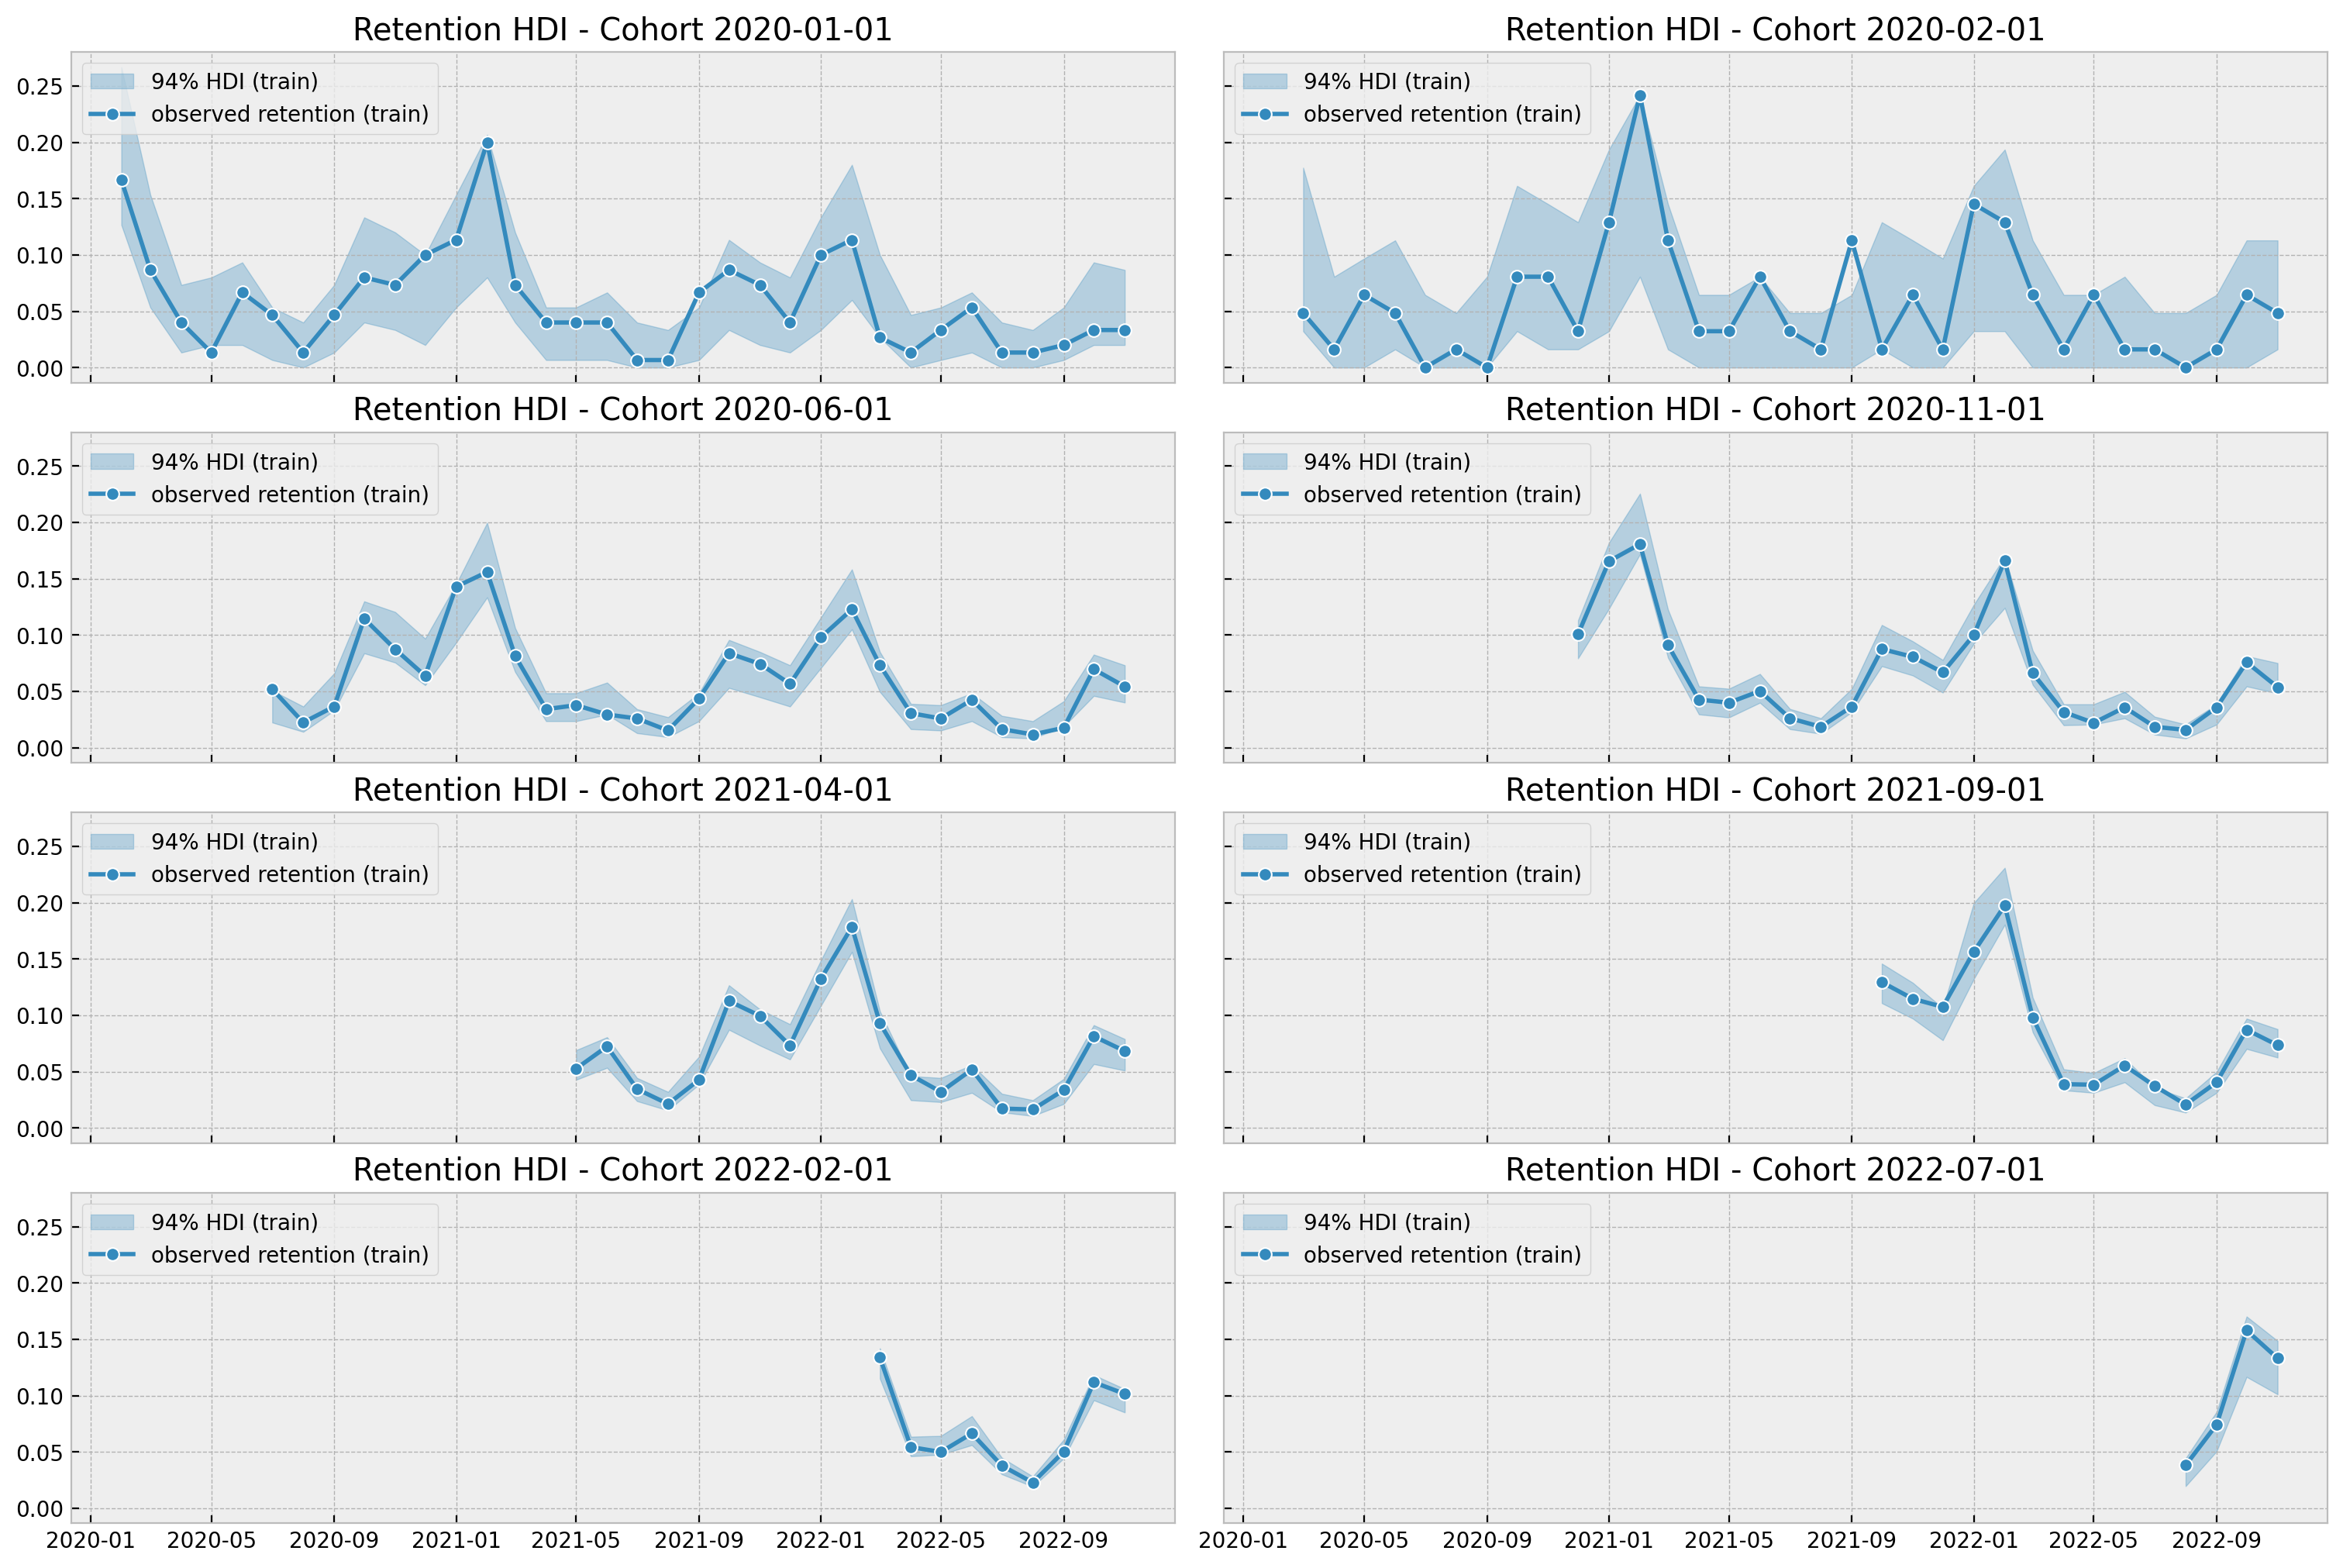
\includegraphics[width=\textwidth]{images/revenue_retention_51_0.png}
\end{figure}

\begin{figure}
    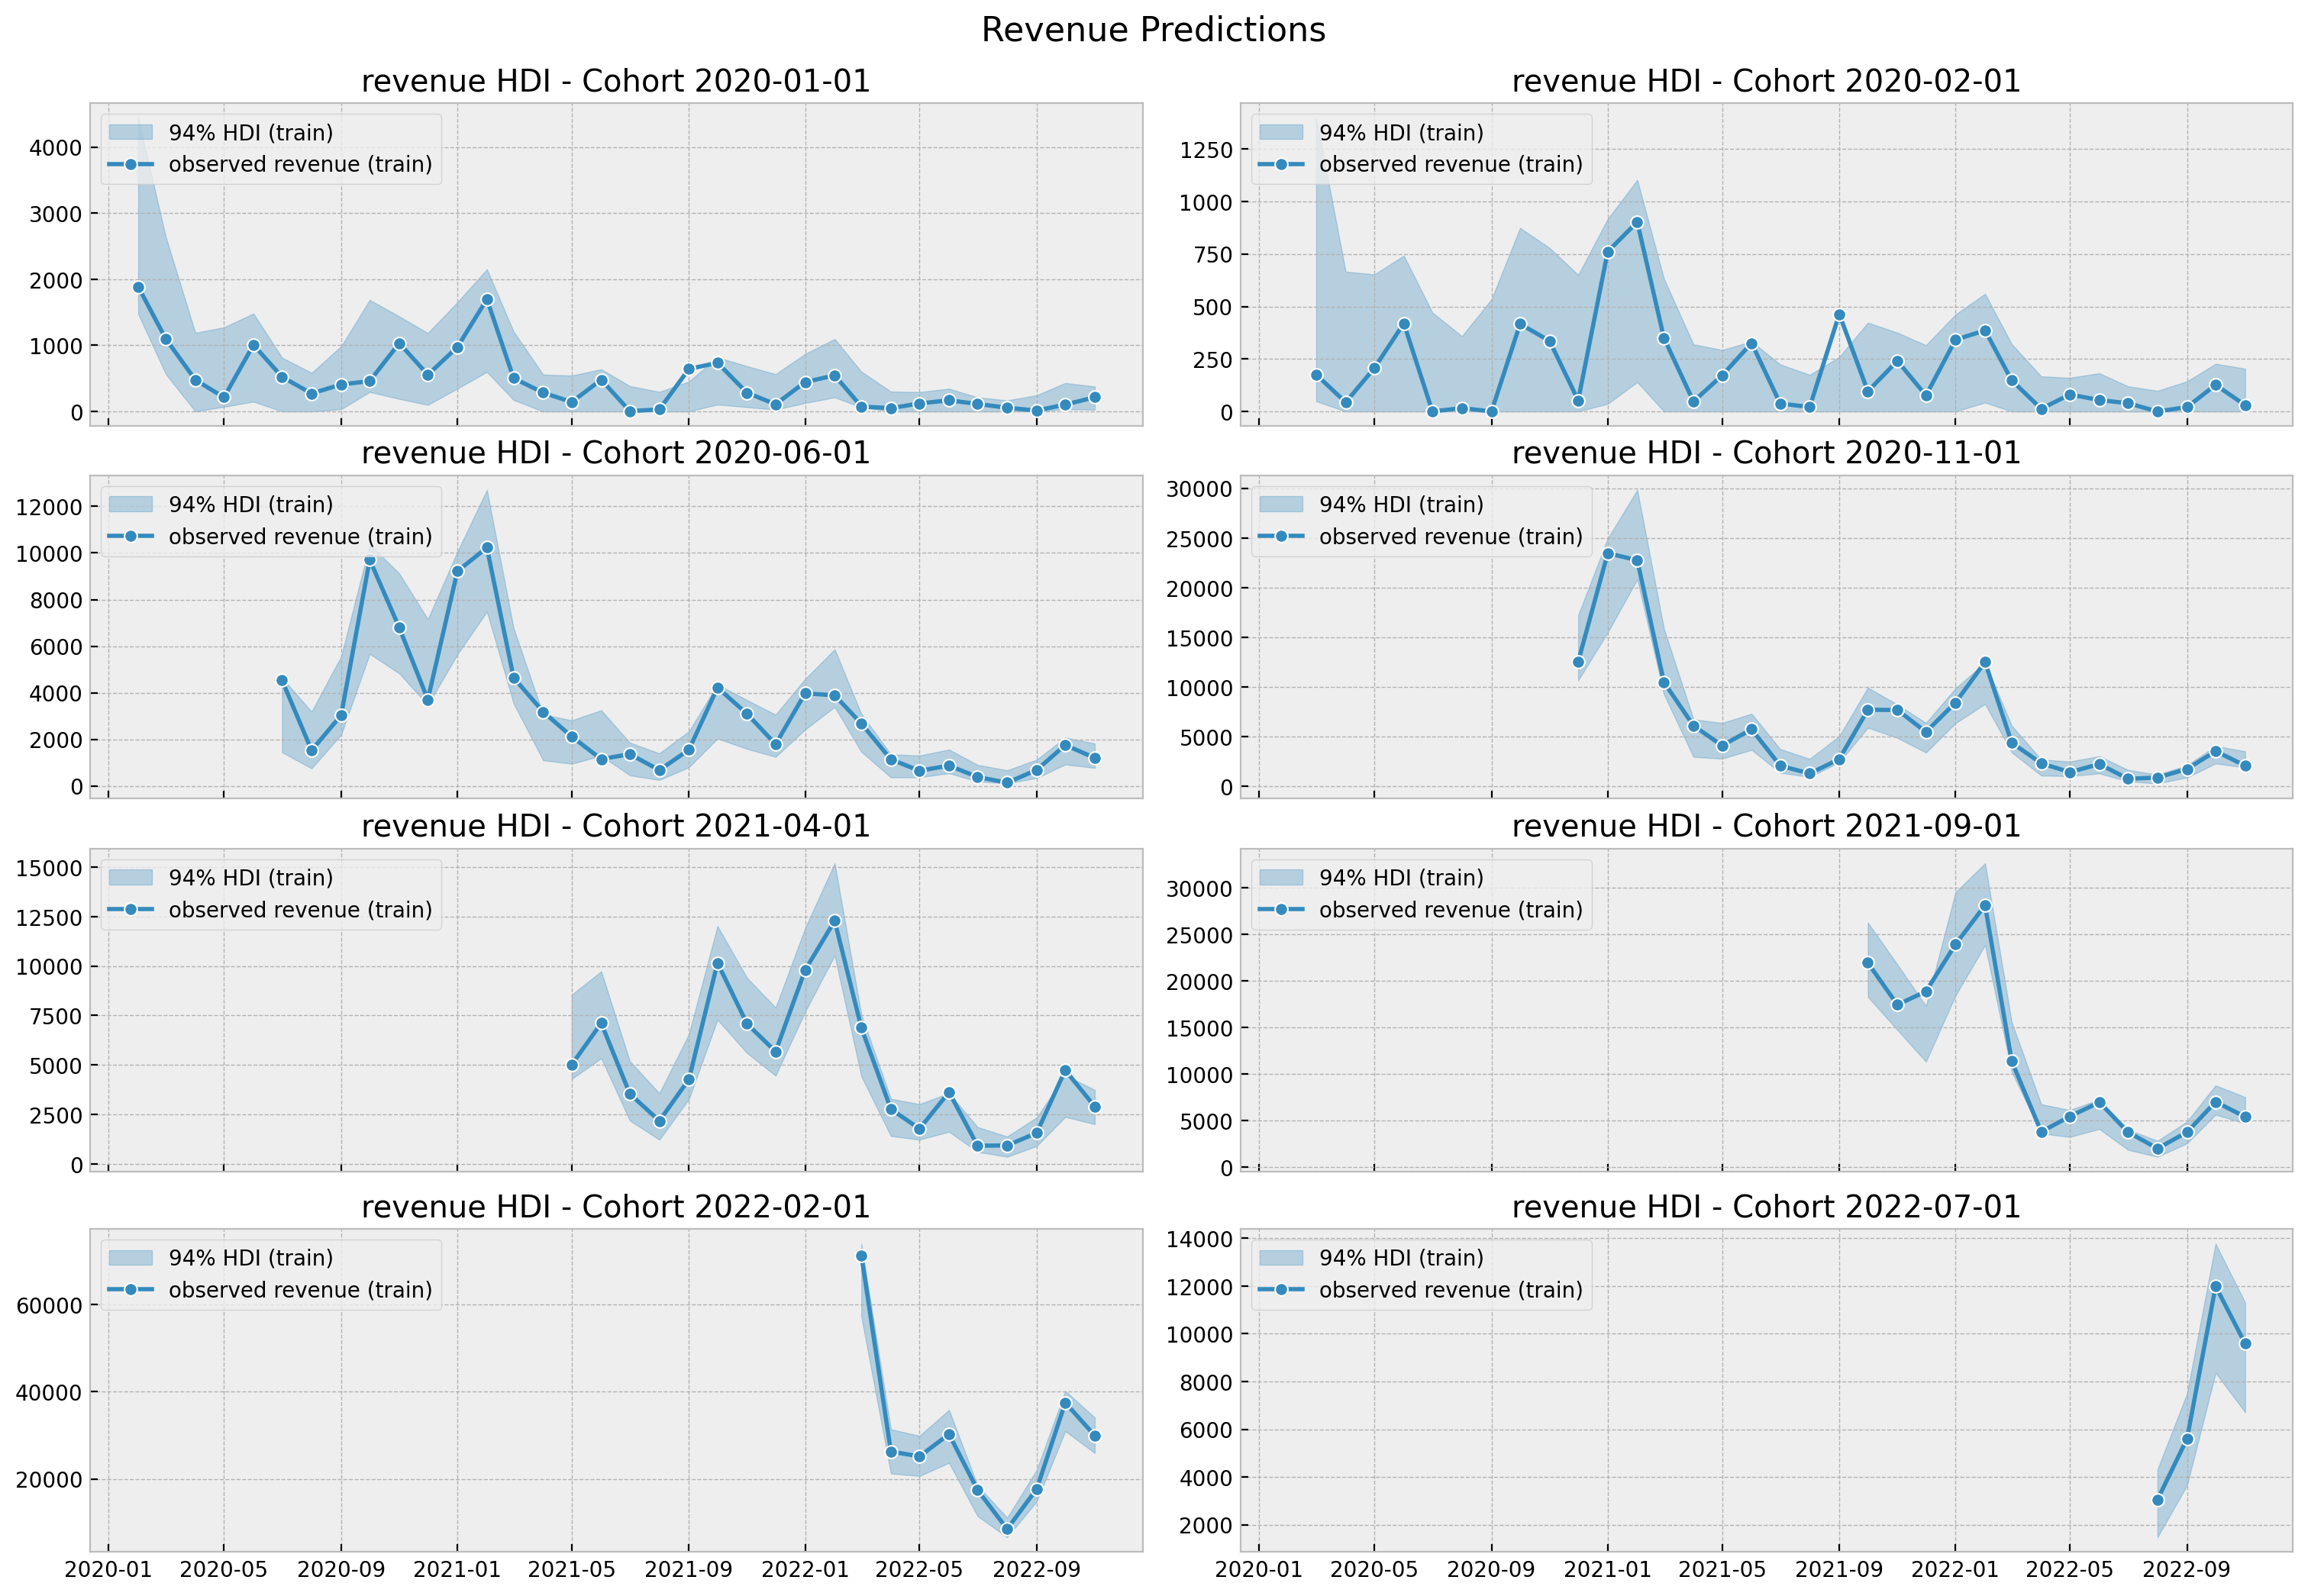
\includegraphics[width=\textwidth]{images/revenue_retention_53_0.png}
\end{figure}

\begin{figure}
    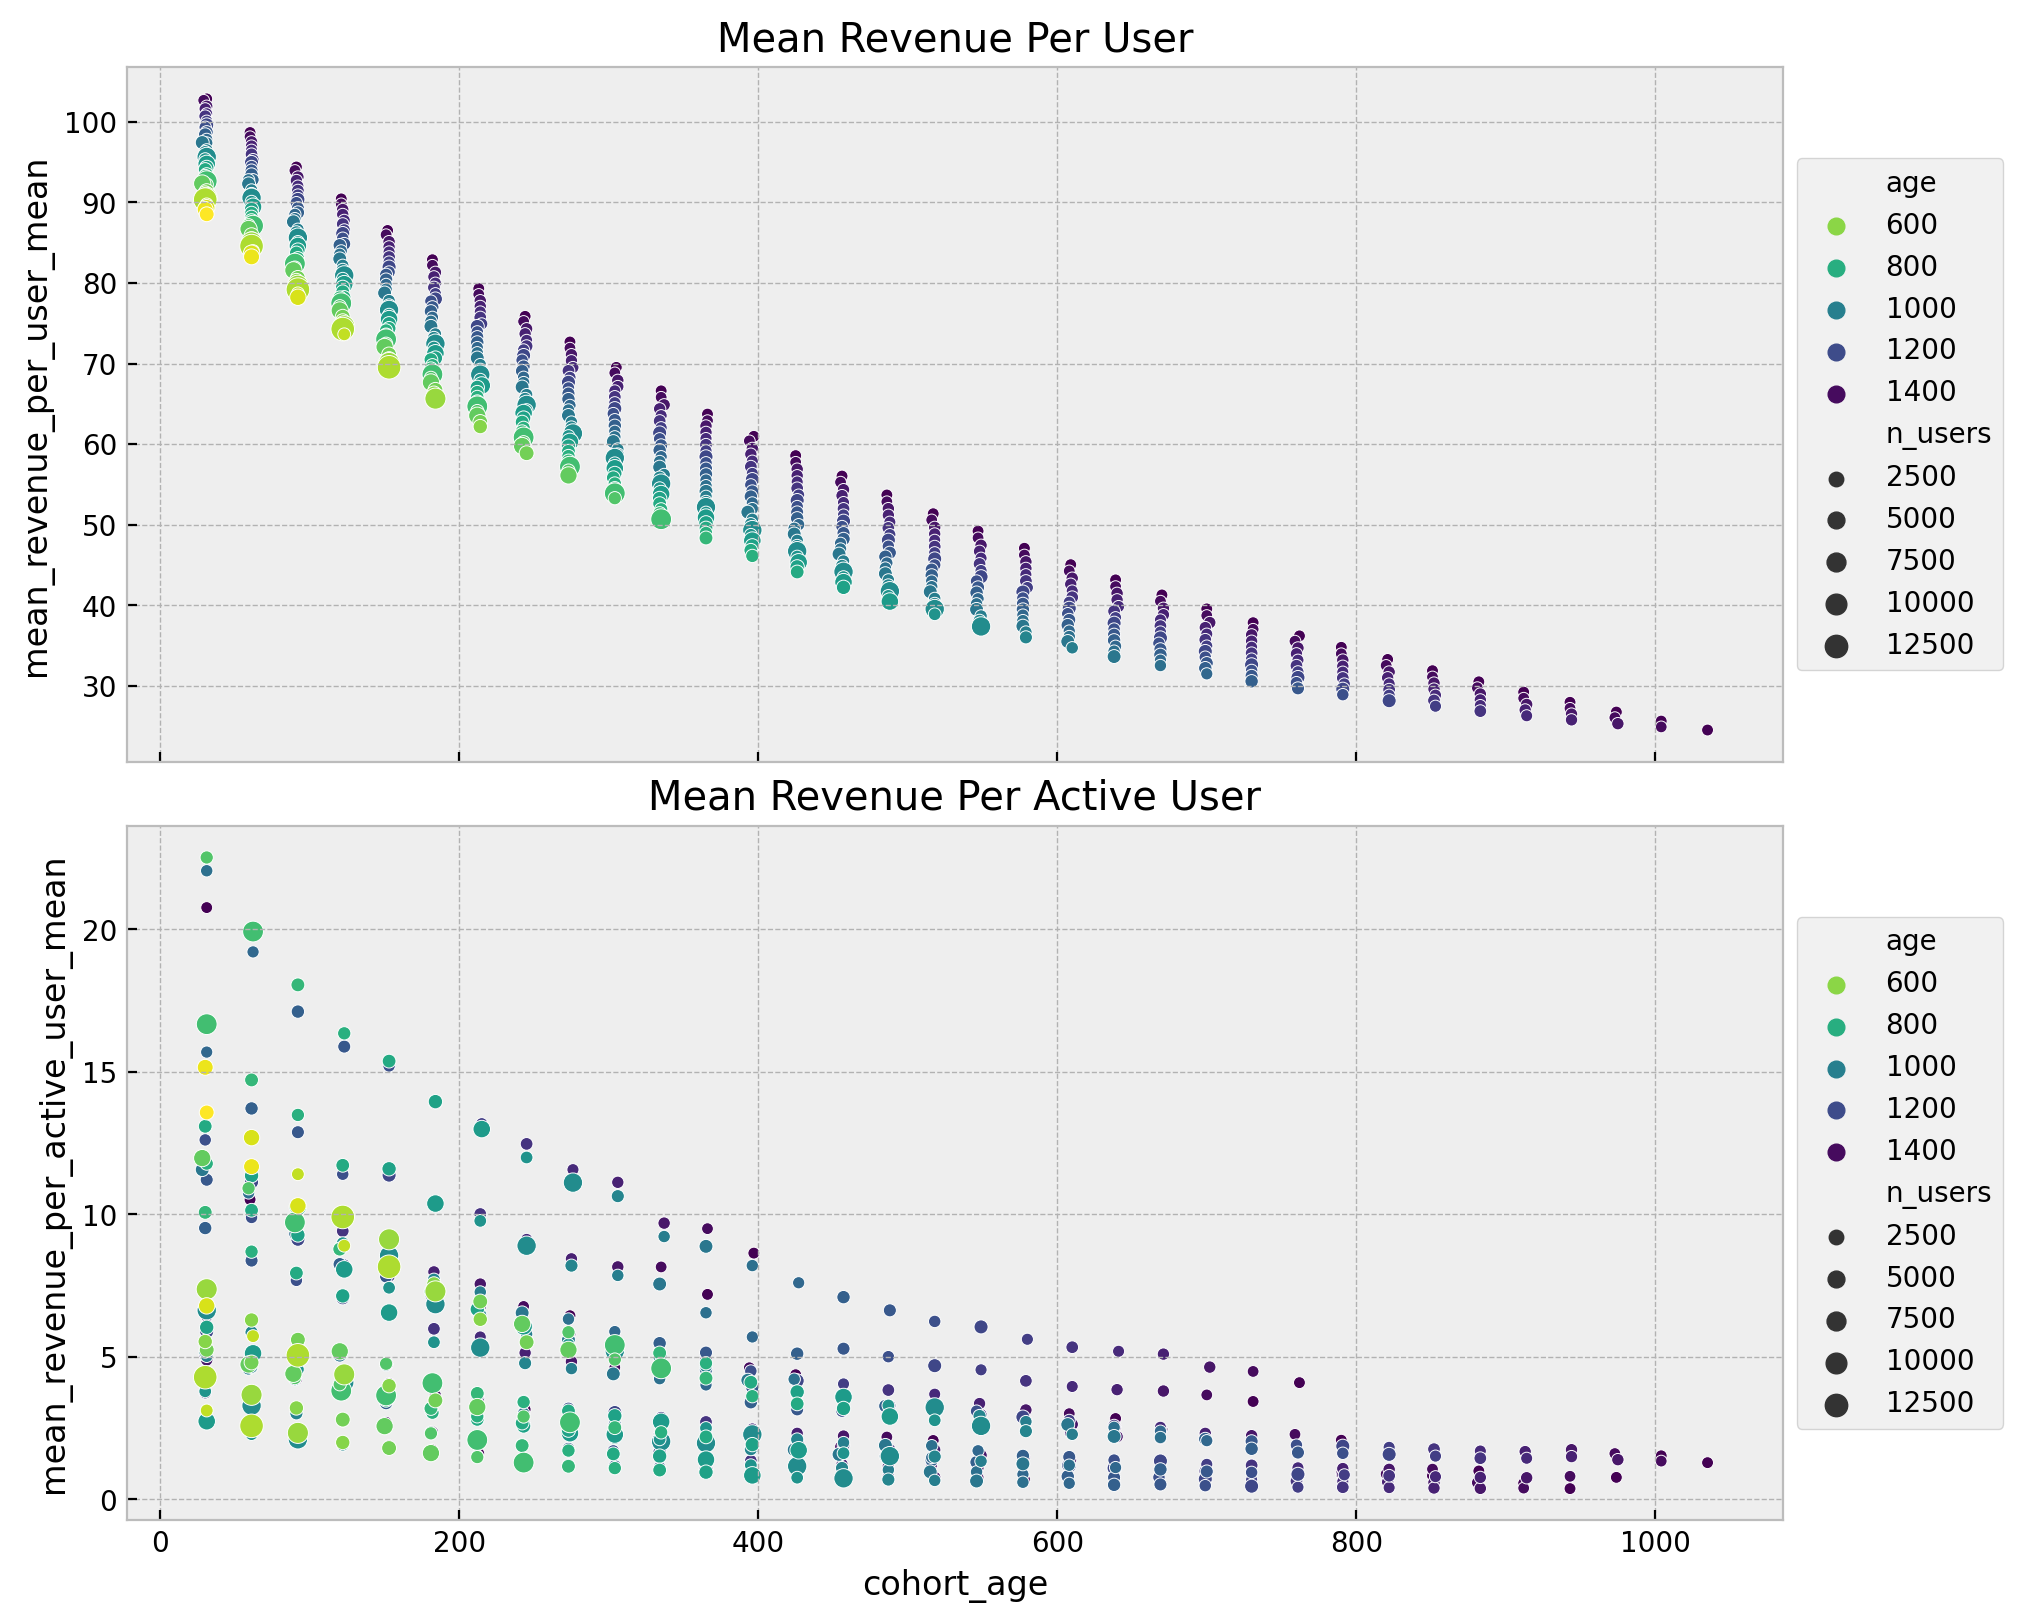
\includegraphics[width=\textwidth]{images/revenue_retention_56_0.png}
\end{figure}

\subsection{Out-of-Sample Predictions}

\begin{figure}
    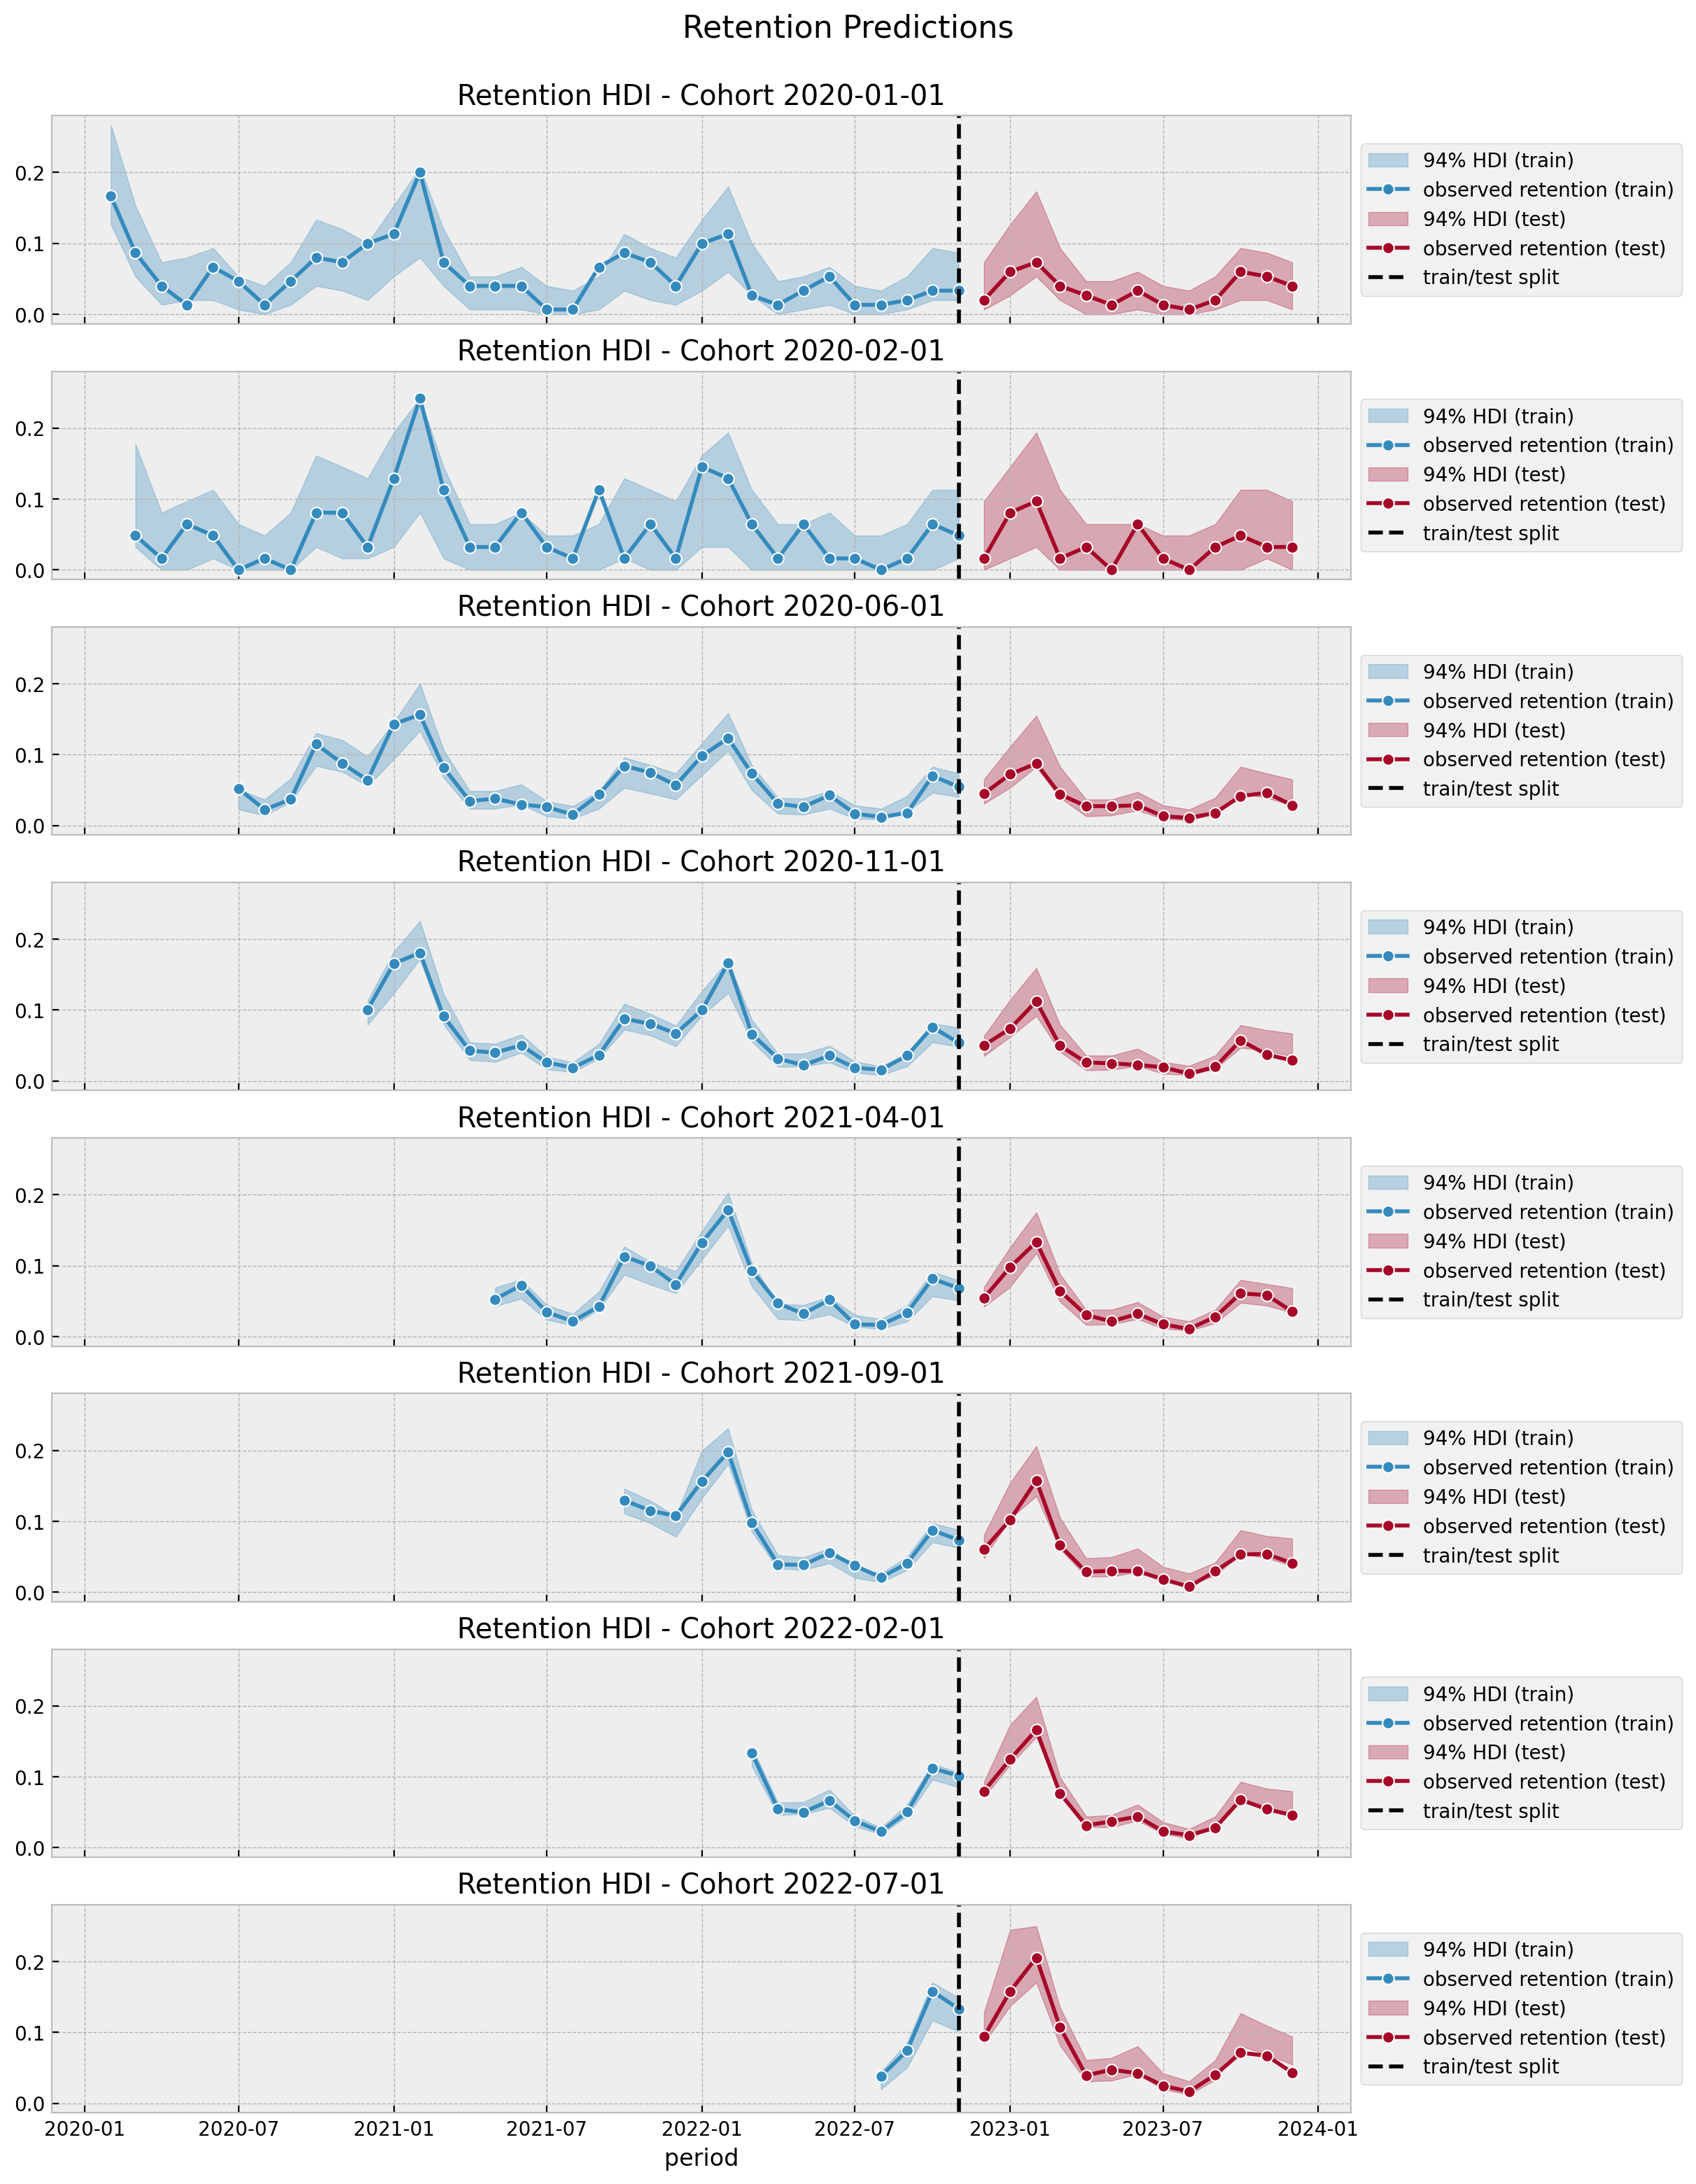
\includegraphics[width=\textwidth]{images/revenue_retention_66_0.png}
\end{figure}

\begin{figure}
    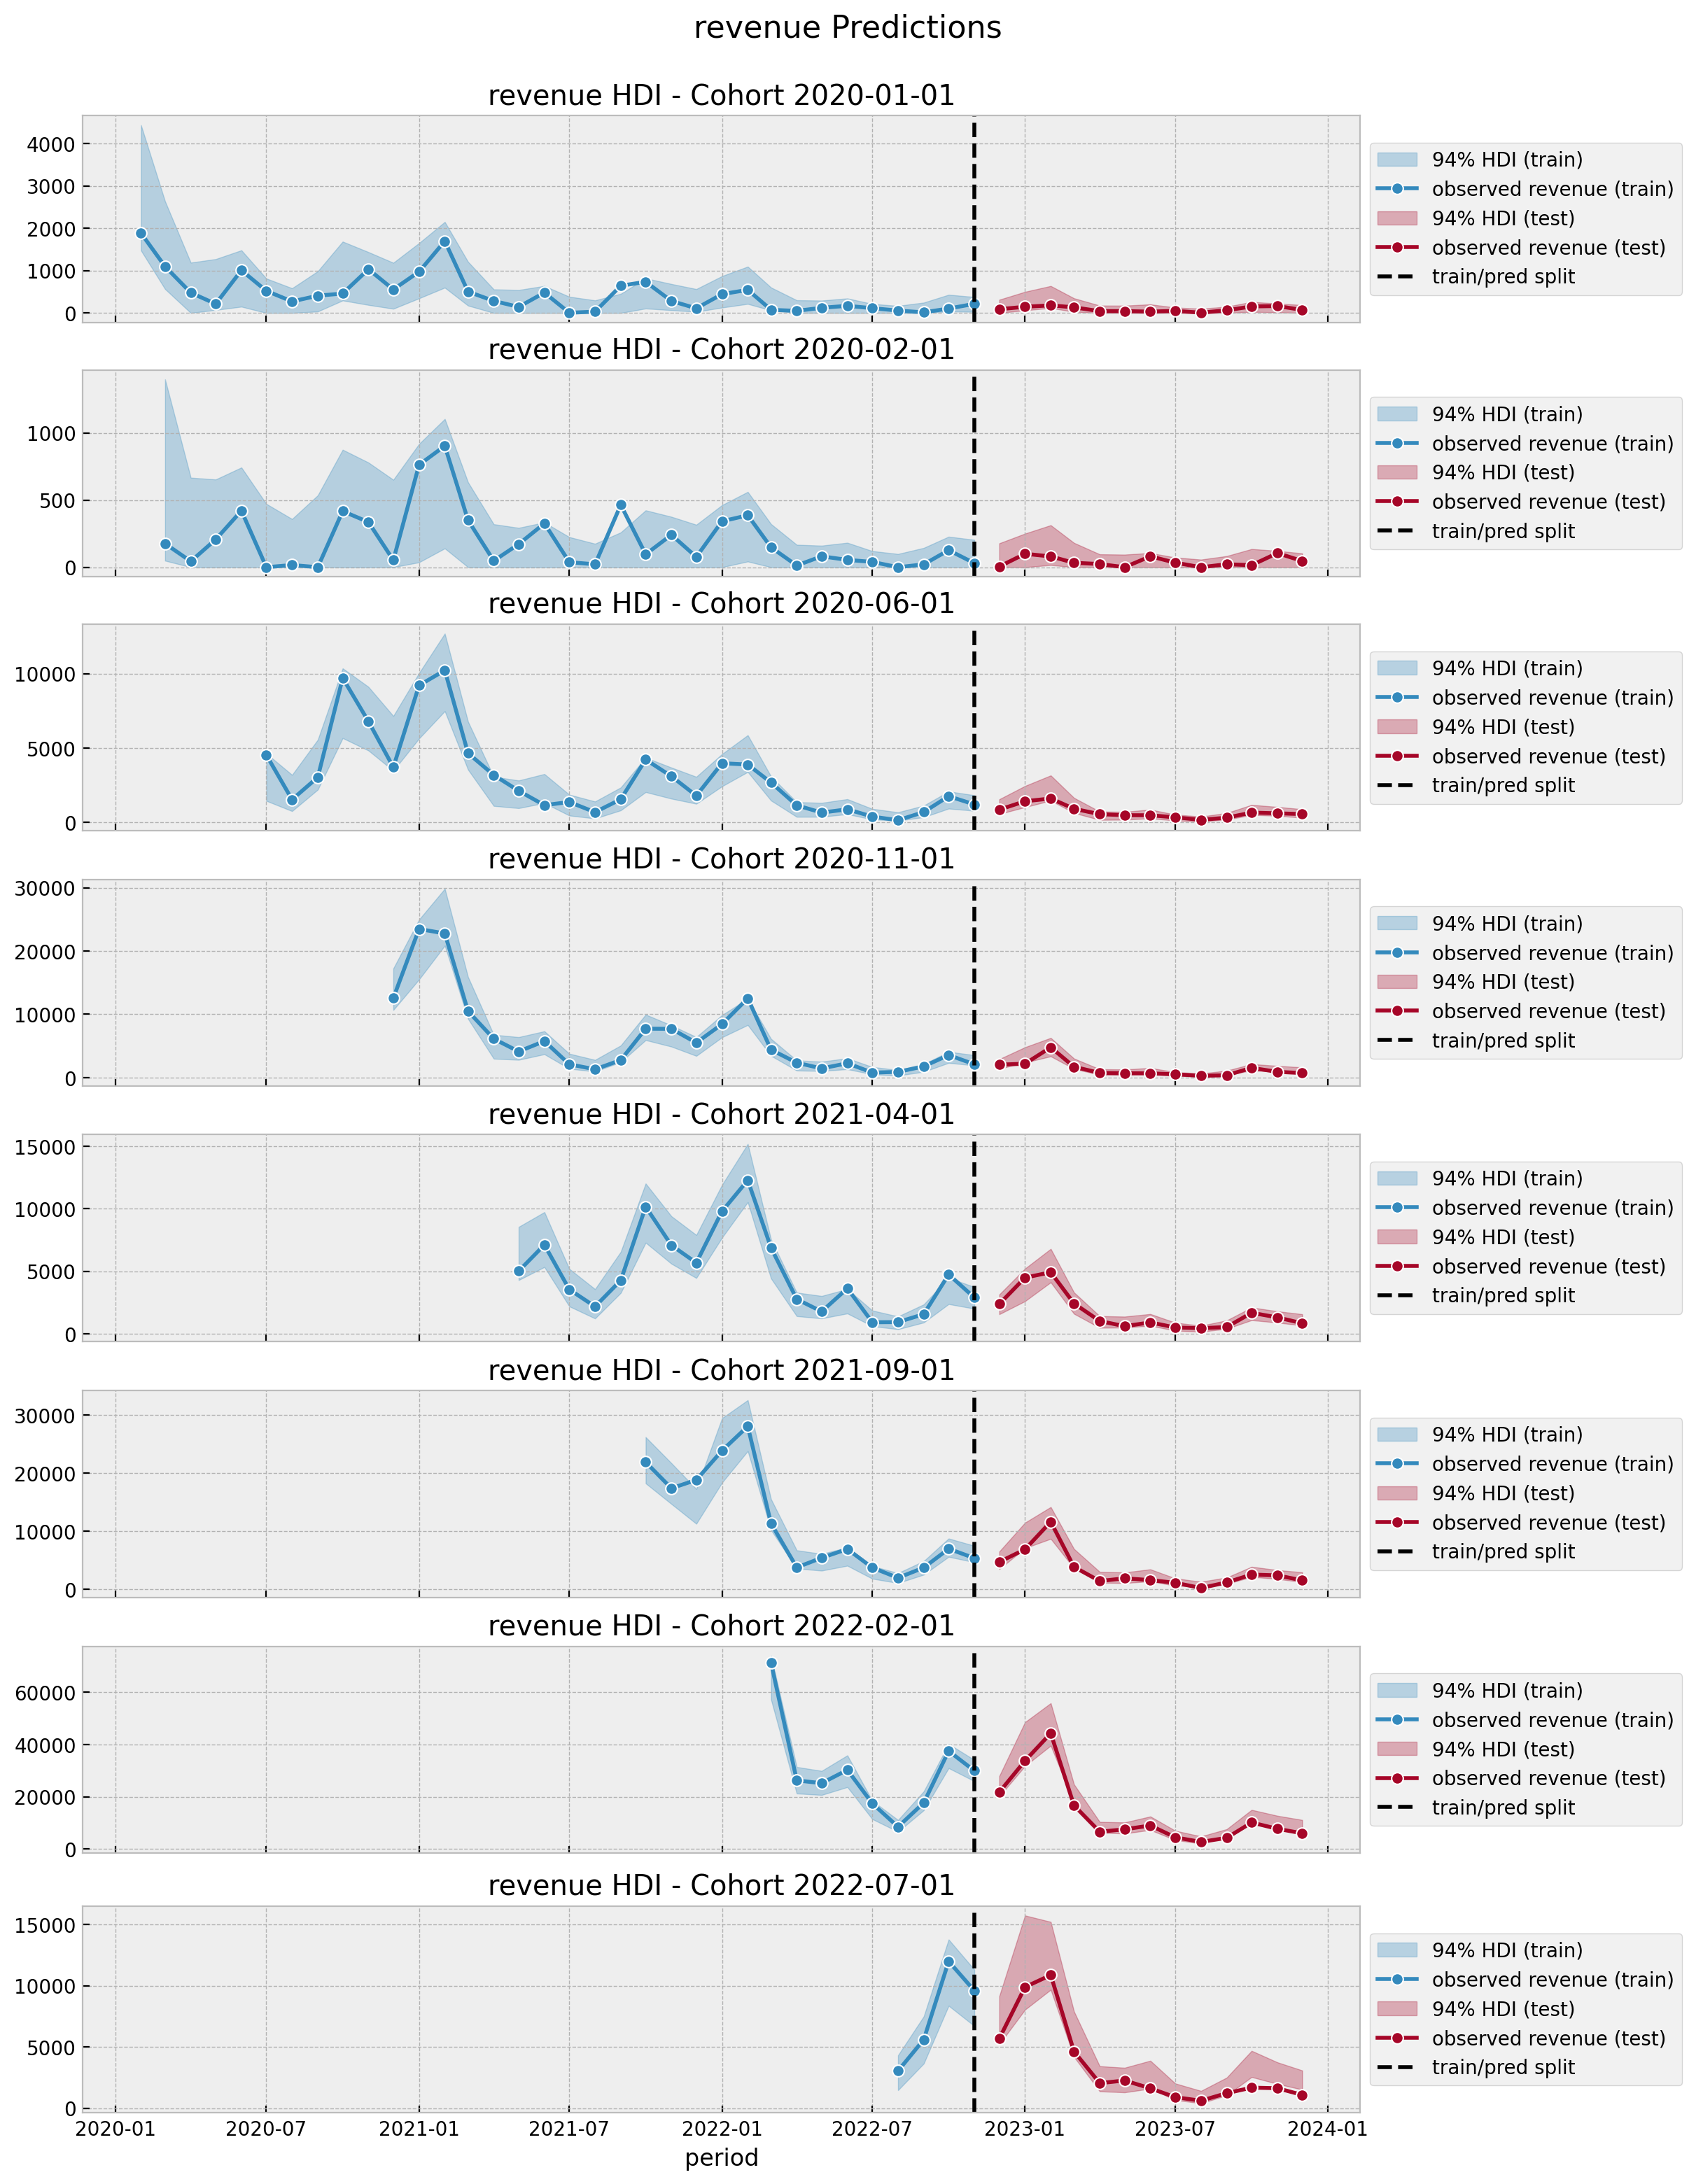
\includegraphics[width=\textwidth]{images/revenue_retention_68_0.png}
\end{figure}

\clearpage

\appendix{Appendix: Python Code}

\begin{lstlisting}[language=Python, caption=Python example]
import pymc_bart as pmb
import pymc as pm


with pm.Model(coords={"feature": features}) as model:

    # --- Data ---
    model.add_coord(name="obs", values=train_obs_idx, mutable=True)
    age_scaled = pm.MutableData(
        name="age_scaled", value=train_age_scaled, dims="obs"
    )
    cohort_age_scaled = pm.MutableData(
        name="cohort_age_scaled", value=train_cohort_age_scaled, dims="obs"
    )
    x = pm.MutableData(name="x", value=x_train, dims=("obs", "feature"))
    n_users = pm.MutableData(name="n_users", value=train_n_users, dims="obs")
    n_active_users = pm.MutableData(
        name="n_active_users", value=train_n_active_users, dims="obs"
    )
    revenue = pm.MutableData(name="revenue", value=train_revenue, dims="obs")

    # --- Priors ---
    intercept = pm.Normal(name="intercept", mu=0, sigma=1)
    b_age_scaled = pm.Normal(name="b_age_scaled", mu=0, sigma=1)
    b_cohort_age_scaled = pm.Normal(name="b_cohort_age_scaled", mu=0, sigma=1)
    b_age_cohort_age_interaction = pm.Normal(
        name="b_age_cohort_age_interaction", mu=0, sigma=1
    )

    # --- Parametrization ---
    # The BART component models the image of the retention rate under the
    # logit transform so that the range is not constrained to [0, 1].
    mu = pmb.BART(name="mu", X=x, Y=train_retention_logit, m=50, dims="obs")
    # We use the inverse logit transform to get the retention rate
    # back into [0, 1].
    p = pm.Deterministic(name="p", var=pm.math.invlogit(mu), dims="obs")
    # We add a small epsilon to avoid numerical issues.
    p = pt.switch(pt.eq(p, 0), eps, p)
    p = pt.switch(pt.eq(p, 1), 1 - eps, p)

    # For the revenue component we use a Gamma distribution where we
    # combine the number of estimated active users with the average
    # revenue per user.
    lam_log = pm.Deterministic(
        name="lam_log",
        var=intercept
        + b_age_scaled * age_scaled
        + b_cohort_age_scaled * cohort_age_scaled
        + b_age_cohort_age_interaction * age_scaled * cohort_age_scaled,
        dims="obs",
    )

    lam = pm.Deterministic(name="lam", var=pm.math.exp(lam_log), dims="obs")

    # --- Likelihood ---
    n_active_users_estimated = pm.Binomial(
        name="n_active_users_estimated",
        n=n_users,
        p=p,
        observed=n_active_users,
        dims="obs",
    )

    x = pm.Gamma(
        name="revenue_estimated",
        alpha=n_active_users_estimated + eps,
        beta=lam,
        observed=revenue,
        dims="obs",
    )

    # --- Derived Quantities ---
    mean_revenue_per_user = pm.Deterministic(
        name="mean_revenue_per_user", var=(1 / lam), dims="obs"
    )
    pm.Deterministic(
        name="mean_revenue_per_active_user",
        var=p * mean_revenue_per_user,
        dims="obs"
    )
\end{lstlisting}



\bibliographystyle{acm}
\bibliography{references}

\end{document}